\let\texyear\year
\documentclass{ieeeaccess}
\let\ieeeaccessyear\year
\let\year\texyear

\usepackage{cite}
\usepackage{amsmath,amssymb,amsfonts,mathtools}
\usepackage{amsthm}
\usepackage{algorithmic}
\usepackage{graphicx}
\usepackage{textcomp}
\usepackage{booktabs}
\usepackage{array}
\usepackage{enumitem}
\usepackage{xcolor}
\usepackage{url}
\usepackage{xspace}
\usepackage{comment}
\usepackage{tikz}
\usepackage{float}
\usepackage[caption=false]{subfig}
\usepackage{expl3}
\usepackage{xparse}
\usetikzlibrary{arrows.meta,shapes,automata,positioning,calc,fit,tikzmark,decorations.pathreplacing,decorations.markings}
% Unified monochrome figure style for the paper.
% All automata and timing diagrams use white states, black borders and black arrows.
\tikzset{
  fmstate/.style={
    circle, draw=black, fill=white, line width=0.6pt,
    minimum size=9mm, inner sep=1pt, font=\small
  },
  fmstatewide/.style={
    rounded rectangle, draw=black, fill=white, line width=0.6pt,
    minimum height=8mm, inner xsep=3pt, inner ysep=1.5pt, font=\small
  },
  fmaccept/.style={fmstate,double,double distance=1.2pt},
  fmerror/.style={fmstate,double,double distance=1.2pt,fill=gray!12},
  fmedge/.style={->,>=Stealth,line width=0.6pt},
  fmlabel/.style={font=\scriptsize,align=center,fill=white,inner sep=1.2pt},
  fminvariant/.style={font=\scriptsize,align=center},
  fmnote/.style={font=\scriptsize,align=center},
  fmtimeline/.style={->,>=Stealth,line width=0.6pt},
  fmevent/.style={circle,draw=black,fill=white,line width=0.6pt,minimum size=4.5mm,inner sep=0.5pt},
  fmreference/.style={fmevent,double,double distance=0.8pt},
  fmguide/.style={densely dashed,line width=0.45pt},
  fmbrace/.style={decorate,decoration={brace,amplitude=4pt},line width=0.5pt}
}


\providecommand{\Nat}{\mathbb{N}}
\providecommand{\Real}{\mathbb{R}}
\providecommand{\CVal}{\mathsf{val}}
\providecommand{\Val}{\mathsf{val}}
\providecommand{\Inv}{\mathit{Inv}}
\providecommand{\T}{\mathcal{T}}
\providecommand{\hEventually}{\widehat{\Diamond}}
\providecommand{\hAlways}{\widehat{\Box}}
\providecommand{\optimize}{\mathsf{optimize}}
\providecommand{\export}{\mathsf{export}}
\newtheorem{theorem}{Theorem}[section]
\newtheorem{lemma}[theorem]{Lemma}
\newtheorem{proposition}[theorem]{Proposition}
\newtheorem{corollary}[theorem]{Corollary}
\newtheorem{assumption}[theorem]{Assumption}
\newtheorem{definition}[theorem]{Definition}
\bibliographystyle{IEEEtran}
\let\year\ieeeaccessyear

\begin{document}
\history{}
\doi{}

\title{Mechanically Verified Optimization and UPPAAL-Oriented Transformation of Timed B\"uchi Automata}
\author{\uppercase{Elie Fares}\authorrefmark{1},
\uppercase{Jean-Paul Bodeveix}\authorrefmark{2},
\uppercase{Hussain Al-Aqrabi}\authorrefmark{1} AND
\uppercase{Azar Salami}\authorrefmark{1}}
\address[1]{Higher Colleges of Technology\\Sharjah, United Arab Emirates\\(e-mail: efares@hct.ac.ae, halaqrabi@hct.ac.ae, asalami@hct.ac.ae)}
\address[2]{IRIT, UPS, Universit\'e de Toulouse, France (e-mail: bodeveix@irit.fr)}

\begin{abstract}
Timed B\"uchi automata (TBAs) produced by translators or other tools can contain redundant timing constraints, resets, transitions, clocks, and locations, and may have disjunctive invariants that require transformation for UPPAAL-oriented use. We present a Rocq-verified pipeline that synthesizes and propagates timing bounds, removes contradictory transitions and dead resets, merges synchronously reset clocks and equivalent transitions and locations, and transforms the result to conjunctive guards and invariants. Every pass preserves the timed-word language of each input TBA under existential initial-clock semantics. The preservation theorems hold for every TBA represented by the formula-indexed clock interface, independently of whether the automaton was generated by the MTL translator. Optimization preserves language for every finite number of rounds; export preserves language and proves structural properties of the internal target representation. The functions are extracted to OCaml and used in \texttt{mtl2tba}; XML printing and its correspondence to UPPAAL are outside the Rocq theorem. Of 31 attempted upstream-generated configurations, 29 produced optimizer inputs. We also evaluate 16 translator-independent synthetic TBAs and four system configurations. Optimization reduces transitions on the completed inputs, while explicit export can increase edge counts. These benchmark-specific results do not establish a universal efficiency gain.
\end{abstract}
\begin{keywords}
Rocq, formal verification, program extraction, timed automata, timed B\"uchi automata, UPPAAL, verified optimization.
\end{keywords}
\titlepgskip=-15pt
\maketitle

\section{Introduction}
\label{sec:introduction}
Timed B\"uchi automata (TBAs) are a common intermediate representation for real-time requirements and are also used as inputs to timed-language analysis tools. An automaton that is correct at the language level may still be inconvenient for downstream verification: its transition guards can repeat constraints, some resets may never affect a future guard, multiple clocks may evolve in lockstep, and the same behavior may be represented by many transitions. In addition, merging transitions can produce disjunctive guards and invariants, while UPPAAL-oriented automata are most useful with conjunctive guards and conjunctive upper-bound invariants.

An optimization pass is safe only when it preserves accepted timed words, including the treatment of clock resets, event labels, and B\"uchi acceptance. Several passes also interact. Propagating a lower bound may make a transition contradictory, but a synthetic nonnegativity guard can keep an otherwise dead clock live unless guards are normalized before reset analysis. Splitting a disjunctive invariant into copies also requires a condition on entry: choosing a copy whose invariant admits less time than another copy can change the accepted language.

This paper presents a mechanically verified post-processing and export pipeline for TBAs. The preservation theorems hold for every TBA represented by the formula-indexed clock interface, independently of whether the automaton was generated by the MTL translator. In this interface, clocks are named by the timed subformulas of a fixed formula; the formula only supplies clock names, and no proof of an optimization or export pass uses any other property of it. In Rocq (formerly Coq), we prove that each optimization and export operation preserves the automaton's timed-word language under the acceptance semantics formalized in the development. The optimizer theorem holds for every finite number of rounds, so the implementation can stop after reaching a structural fixed point or after its configured iteration bound without relying on convergence for correctness.

The transformations have two stages. The optimization stage synthesizes upper-bound location invariants, propagates target invariants backward into guards, propagates entry lower bounds forward, removes contradictory and unreachable transitions, removes dead resets, merges clocks reset synchronously, tightens guards, and merges transitions and locations. The export stage merges transitions with equal source, target, label, and resets; eliminates disjunctive invariants by creating copies with conjunctive invariants and clock-difference entry conditions; splits disjunctive guards; normalizes the result; and emits symbolic transitions for drawing.

The verified transformations are extracted to OCaml and used by \texttt{mtl2tba}. Our earlier article~\cite{fares_bodeveix_mtl_translation} establishes the correctness of a specified MTL$_{0,\infty}$-to-TBA translation. Its output may still contain redundant bounds, resets, clocks, transitions, and locations, and may not have the invariant shape needed for UPPAAL-oriented output. This paper begins with that TBA and verifies the later optimization and representation transformations. The preservation theorems quantify over every TBA in the formal input type, irrespective of provenance; that proof scope does not supply a verified parser for arbitrary third-party formats. Our evaluation includes both upstream-generated inputs and a separate translator-independent synthetic suite, and we keep those evidence sources distinct.

The contributions are:
\begin{itemize}[leftmargin=*]
  \item a Rocq development of language-preserving TBA transformations, including invariant synthesis and propagation, clock and state simplification, transition merging, and disjunctive-invariant elimination;
  \item a preservation theorem for every TBA of the formula-indexed clock interface and every number of optimization rounds, plus a verified export composition whose final guards and invariants are conjunctive;
  \item an extracted implementation and an explicit account of its interface and trust boundaries; and
  \item a reproducible evaluation on 29 completed optimizer inputs from 31 attempted upstream-generated configurations, 16 directly constructed TBA records designed to exercise the passes, and four system-model configurations, with the input-generation and measurement boundaries stated explicitly.
\end{itemize}
Our earlier article, ``A Mechanically Verified Translation of MTL$_{0,\infty}$ into Timed B\"uchi Automata''~\cite{fares_bodeveix_mtl_translation}, establishes the source translation theorem, and this paper reuses its Rocq core and correctness files unchanged. The present paper starts from the resulting TBA and verifies the subsequent optimization and export transformations. The composition theorem in Section~\ref{sec:composition} retains the backend-language contract as a hypothesis; neither the Spot executable nor the XML printer is covered by that theorem.

\section{Timed Automata and the Preservation Contract}
\label{sec:model}
\subsection{Timed words and TBAs}
A timed word is an infinite sequence $w=(a_i,t_i)_{i\in\Nat}$, where $a_i$ is an event from a finite alphabet $\Sigma$, timestamps satisfy $t_i\ge0$ and are strictly increasing, and time diverges: $\lim_{i\to\infty}t_i=+\infty$. For each position $i$, let $\delta_i=t_{i+1}-t_i$ be the time from event $i$ to the next event. A clock valuation maps a finite clock set $X$ to $\Real_{\ge0}$. Guards are finite conjunctions of event literals and clock comparisons $x\bowtie c$ for $\bowtie\in\{<,\le,=,\ge,>\}$; transitions also carry a set of clocks to reset.

A TBA is a tuple $\mathcal A=(L,\ell_0,X,E,\mathit{Acc})$, where $L$ is a finite location set, $\ell_0$ is the initial location, $X$ is the clock set, $E$ is a finite set of transitions $(\ell,\alpha,g,Z,\ell')$, $\alpha$ is an event condition, $g$ is a clock guard, $Z\subseteq X$ is a reset set, and $\mathit{Acc}\subseteq L$ is the set of B\"uchi-accepting locations. The starting automata in the verified optimization are represented without location invariants; synthesis adds them as a separate annotation. Exported invariants are conjunctions of upper bounds.

The Rocq development interprets transitions over an extended timed word that records clock values and reset decisions. Here $v_i$ is the clock valuation at event $i$, and $Z_i$ records the clocks reset by the transition on that event. Since a reset occurs at $t_i$, the next-event valuation includes the elapsed interval $\delta_i$:
\[
v_{i+1}(x)=
\begin{cases}
\delta_i,&x\in Z_i,\\
v_i(x)+\delta_i,&x\notin Z_i.
\end{cases}
\]
A run chooses one enabled transition per position and visits accepting locations infinitely often. The accepted language existentially quantifies over clock-consistent extensions of the base timed word, including the initial clock values. This is the acceptance notion of the preservation theorems; conventional initialization at zero is a separate deployment concern.

For an annotated automaton, an invariant must hold throughout the delay spent at its location. Since synthesized invariants are conjunctions of non-strict upper bounds and clocks are nondecreasing during a delay, holding at the event at the end of the delay is equivalent to holding throughout that stay. The proof formalizes this trace-model equivalence and uses it to show that the annotations and strengthening operations preserve timed words.

\subsection{What export must preserve}
\label{sec:export-contract}
The export must retain the same transition alphabet, B\"uchi marking, clock meaning, and timed-word language. It may change the number of locations, transitions, and clocks, and may introduce difference constraints in transition guards to choose among invariant copies. Such choices must not create or delete an accepted timed word. The target representation has conjunctive guards and conjunctive location invariants; a later symbolic representation groups transitions with identical source, target, and reset sets under Boolean labels.

The preservation theorems hold for every TBA represented by the formula-indexed clock interface, independently of whether the automaton was generated by the MTL translator. Their proof does not require properties of the MTL translation or Spot. An upstream correctness theorem can be composed with these results, but Spot's correctness and the soundness of the front end are outside the pass theorems.

\section{Verified Optimization}
\label{sec:post}
After invariant synthesis, the optimization pipeline alternates timing propagation with simplification. Synthesized upper bounds expose how long an automaton can remain at a location. Propagating them to incoming guards can make lower and upper constraints jointly inconsistent; forward propagation supplies complementary lower-bound information. The pipeline then removes transitions, resets, clocks, and duplicate structure that no longer affect the language.

\begin{table*}[t]
\centering
\caption{Verified post-processing passes. Each preservation theorem quantifies over every input TBA under the Rocq timed-word semantics. Detailed definitions and proof arguments follow in this section.}
\label{tab:post-passes}
\small
\begin{tabular}{@{}p{0.42\textwidth}p{0.52\textwidth}@{}}
\toprule
Pass & Rocq preservation theorem\\
\midrule
Upper-bound invariant synthesis & \path{add_invariants_accepts}\\
Backward propagation ($n$ steps) & \path{propagate_n_accepts}\\
Forward propagation of lower bounds & \path{forward_accepts}\\
Two-sided invariants & \path{add_two_sided_invariants_accepts}\\
Removal of contradictory transitions & \path{remove_contradictory_accepts}\\
Removal of outgoing transitions from locations with no incoming transition & \path{remove_unreachable_accepts}\\
Removal of dead resets & \path{remove_dead_resets_accepts}\\
Merging synchronously reset clocks & \path{merge_all_accepts}\\
Normalization of guards & \path{normalize_accepts}\\
Removal of unsatisfiable action labels & \path{remove_unsat_accepts}\\
Merging transitions & \path{merge_trans_accepts}\\
Merging equivalent locations & \path{merge_states_all_accepts}\\
Iterated pipeline ($n$ rounds) & \path{optimize_accepts}\\
Merging transitions for export & \path{merge_transitions_accepts}\\
Maximal-delay invariant split & \path{split_accepts}, \path{split_inv_conjunctive}\\
All-copy invariant split & \path{split_all_accepts}, \path{split_all_inv_conjunctive}\\
Splitting of disjunctive guards & \path{explode_accepts}\\
Normalization of exported guards & \path{normalize_d_accepts}\\
Removal of copies never entered & \path{dprune_n_accepts}\\
Merging of the initial location & \path{dmerge_states_all_accepts}\\
Symbolic transitions & \path{symbolic_ext_accepts}\\
Complete export & \path{export_accepts}; shape: \path{export_guards_conjunctive}, \path{export_invariants_conjunctive}\\
All-copy export & \path{export_all_accepts}; shape: \path{export_all_guards_conjunctive}, \path{export_all_invariants_conjunctive}\\
\bottomrule
\end{tabular}
\end{table*}

\begin{figure}[t]
\centering
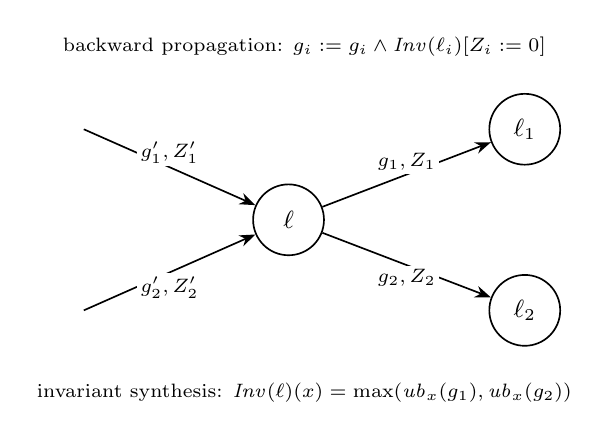
\begin{tikzpicture}[node distance=20mm]
  \node[fmstate] (L) at (0,0) {$\ell$};
  \node[fmstate] (S1) at (3.0,1.15) {$\ell_1$};
  \node[fmstate] (S2) at (3.0,-1.15) {$\ell_2$};
  \coordinate (P1) at (-2.6,1.15);
  \coordinate (P2) at (-2.6,-1.15);
  \draw[fmedge] (P1) -- node[fmlabel,above] {$g'_1,Z'_1$} (L);
  \draw[fmedge] (P2) -- node[fmlabel,below] {$g'_2,Z'_2$} (L);
  \draw[fmedge] (L) -- node[fmlabel,above] {$g_1,Z_1$} (S1);
  \draw[fmedge] (L) -- node[fmlabel,below] {$g_2,Z_2$} (S2);
  \node[fmnote] at (0.20,2.20) {backward propagation: $g_i:=g_i\land \mathit{Inv}(\ell_i)[Z_i:=0]$};
  \node[fmnote] at (0.20,-2.20) {invariant synthesis: $\mathit{Inv}(\ell)(x)=\max(\mathit{ub}_x(g_1),\mathit{ub}_x(g_2))$};
\end{tikzpicture}

\caption{Invariant computation. Successor invariants strengthen outgoing
guards; upper bounds of the resulting guards resynthesize the source
invariant. Reset sets determine which target-clock constraints become
constant.}
\label{fig:main-inv-unified}
\end{figure}

\subsection{Location invariants on the trace model}
\label{sec:inv-semantics}
A location invariant maps every clock $x$ either to an upper bound
$M\in\mathbb R$, standing for the constraint $x\le M$, or to $+\infty$ (no
constraint).  We interpret automata with invariants on the extended words of
Section~\ref{sec:model}, as we do for automata without invariants.
Along a run $r$, the automaton stays in location $r(i)$ between the events
$i-1$ and $i$, and the invariant of $r(i)$ must hold during the whole stay,
that is, at the clock values $\CVal_\rho(i,x)-\tau$ for every delay
$\tau\in[0,\Delta_{i-1}]$, where $\Delta_{i-1}=t_i-t_{i-1}$ (and at the values $\CVal_\rho(0,x)$ for the
initial location).  This is the condition of Section~\ref{sec:model}, evaluated at
the event that ends the stay.  Since clocks increase while time elapses, an
invariant made of upper bounds holds during the stay if and only if it holds at
the event that ends it (lemma \texttt{inv\_\allowbreak{}during\_\allowbreak{}iff\_\allowbreak{}at\_\allowbreak{}event}).
For the two-sided invariants of Section~\ref{sec:forward}, a lower bound
$x\ge m$ must likewise hold during the whole stay, hence at its beginning.

\subsection{Invariant synthesis and backward propagation}
\label{sec:uppaal-invariants}\label{sec:main-invariants}
In the exported timed automaton, upper-bounded guards need invariants so that
time does not elapse past all useful outgoing transitions.  We compute location
invariants from outgoing upper bounds and propagate successor requirements
backward, using location invariants to constrain admissible time elapse as in
standard UPPAAL models~\cite{[BGD04]}.

\paragraph{Upper bound of a guard.}
For a conjunctive guard $g$ and a clock $x$, let $\mathit{ub}_x(g)$ be the
smallest bound $m$ of the constraints $x\le m$, $x<m$, and $x=m$ occurring in
$g$, and $+\infty$ if $g$ contains none.  Other constraints are ignored.  A
valuation satisfying $g$ satisfies $x\le\mathit{ub}_x(g)$.

\paragraph{Invariant synthesis.}
For a location $\ell$ with outgoing transitions
$\ell\xrightarrow{g_i,Z_i}\ell_i$, $i=1,\dots,m$, the synthesized invariant is
\[
  \mathit{Inv}(\ell)(x)=\max_{1\le i\le m}\mathit{ub}_x(g_i),
\]
with $\mathit{Inv}(\ell)(x)=+\infty$ when $\ell$ has no outgoing transition.
Thus a clock that some outgoing guard does not bound does not appear in the
invariant.  The bound is always non-strict, even when it comes from a strict
guard $x<m$: the invariant only needs to be implied by the guard of the next
transition, and strictness is kept in the guards themselves.

\begin{theorem}[Invariant synthesis]
\label{thm:inv-synthesis}
For every TBA $\mathcal A$, the automaton $\mathcal A$ with the synthesized
invariants accepts the same timed words as $\mathcal A$.
\end{theorem}

\begin{proof}
Adding invariants can only remove runs.  Conversely, let $r$ be an accepting
run on $\rho$.  At every event $i$, the transition taken from $r(i)$ is enabled,
so its guard holds at the values $\CVal_\rho(i,x)$, which are therefore at most
$\mathit{Inv}(r(i))(x)$.  By the lemma \texttt{inv\_\allowbreak{}during\_\allowbreak{}iff\_\allowbreak{}at\_\allowbreak{}event}, the invariant of $r(i)$ holds during
the whole stay.  (Rocq: \texttt{add\_\allowbreak{}invariants\_\allowbreak{}correct}.)
\end{proof}

\paragraph{Backward propagation.}
One propagation step strengthens every transition
$\ell\xrightarrow{g,Z}\ell'$ with the invariant of its target after the
resets:
\[
  g := g\wedge\mathit{Inv}(\ell')[Z:=0],
\]
where $\mathit{Inv}(\ell')[Z:=0]$ replaces every bound $x\le M$ on a reset clock
$x\in Z$ by the constant constraint $0\le M$, that is, by $\top$ if $M\ge0$ and
by $\bot$ otherwise.  Invariants are then synthesized again from the
strengthened guards.

\begin{theorem}[Backward propagation]
\label{thm:propagation}
For every TBA $\mathcal A$ and every $n\in\Nat$, the automaton obtained by
$n$ propagation steps accepts the same timed words as $\mathcal A$.
\end{theorem}

\begin{proof}
Strengthening guards can only remove runs.  Conversely, consider an accepting
run that takes $\ell\xrightarrow{g,Z}\ell'$ at event $i$ and then a transition
$\ell'\xrightarrow{g',Z'}\ell''$ at event $i+1$.  The second guard holds at event
$i+1$, so the values at that event are bounded by $\mathit{Inv}(\ell')$.  Clock
consistency gives $\CVal_\rho(i+1,x)=\Delta_i$ for $x\in Z$ and
$\CVal_\rho(i+1,x)=\CVal_\rho(i,x)+\Delta_i\ge\CVal_\rho(i,x)$ otherwise; hence
the strengthened guard $g\wedge\mathit{Inv}(\ell')[Z:=0]$ holds at event $i$.
The argument uses clock consistency, so the theorem is stated on timed words.
(Rocq: \texttt{propagate\_\allowbreak{}accepts} and
\texttt{propagate\_\allowbreak{}n\_\allowbreak{}accepts}.)
\end{proof}

Each round of the optimization pipeline of Section~\ref{sec:main-pipeline}
applies one propagation step.  The tool repeats the rounds until the
automaton is structurally equal to the previous one, as an OCaml value, or
until 50 rounds have been performed; the bound guarantees termination, and the
theorem holds for every number of steps, whether or not a fixed point is
reached. On the 29 completed optimizer inputs, the greatest observed number
of changed rounds is six (R6).
The invariant computation at one location is summarized in the article's
Figure~\ref{fig:main-inv-unified}.

\paragraph{Example.}
We illustrate the algorithm on the automaton of Fig.~\ref{fig:inv-example},
which contains a two-location cycle $\ell_1\to\ell_2\to\ell_1$ and a self-loop
at $\ell_2$.  It has one clock $x$, the initial location $\ell_0$, and the
transitions
\[
\begin{aligned}
&\ell_0 \xrightarrow{a,\;Z=\{x\}} \ell_1,\quad
 \ell_1 \xrightarrow{b,\;x\le 2,\;Z=\emptyset} \ell_2,\\
&\ell_2 \xrightarrow{c,\;\top,\;Z=\emptyset} \ell_1,\quad
 \ell_2 \xrightarrow{d,\;x\le 1,\;Z=\emptyset} \ell_2.
\end{aligned}
\]
The edge $\ell_1\xrightarrow{b}\ell_2$ requires $x\le2$, and the self-loop at
$\ell_2$ requires the tighter bound $x\le1$.

\begin{figure}[t]
\centering
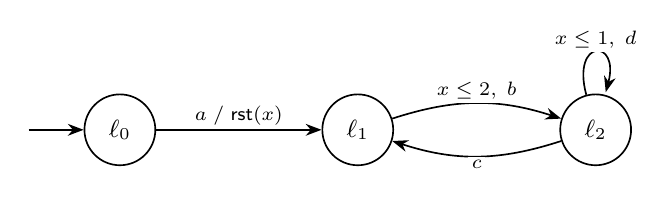
\begin{tikzpicture}[node distance=21mm]
  \node[fmstate] (l0) {$\ell_0$};
  \node[fmstate,right=of l0] (l1) {$\ell_1$};
  \node[fmstate,right=of l1] (l2) {$\ell_2$};
  \draw[fmedge] ([xshift=-7mm]l0.west) -- (l0.west);
  \draw[fmedge] (l0) -- node[fmlabel,above] {$a\;/\;\mathsf{rst}(x)$} (l1);
  \draw[fmedge] (l1) to[bend left=18] node[fmlabel,above] {$x\le2,\;b$} (l2);
  \draw[fmedge] (l2) to[bend left=18] node[fmlabel,below] {$c$} (l1);
  \draw[fmedge] (l2) edge[loop above] node[fmlabel] {$x\le1,\;d$} (l2);
\end{tikzpicture}

\caption{Automaton used to illustrate invariant propagation, with one clock $x$
and actions $a$--$d$.  Edges are labeled ``guard, action / resets'' (the guard
is omitted when it is $\top$); only the edge $\ell_0\to\ell_1$ resets $x$.  The
incoming arrow marks the initial location; acceptance plays no role here.  The
computed fixed point is $\mathit{Inv}(\ell_1)=\mathit{Inv}(\ell_2)=(x\le2)$.}
\label{fig:inv-example}
\end{figure}

\begin{enumerate}
\item \emph{Synthesis.}  $\mathit{Inv}(\ell_1)(x)=\mathit{ub}_x(x\le2)=2$.  At
$\ell_2$, $\mathit{Inv}(\ell_2)(x)=\max(1,+\infty)=+\infty$, because the
transition toward $\ell_1$ does not bound $x$.  At $\ell_0$, the only outgoing
guard is $\top$, so $\mathit{Inv}(\ell_0)(x)=+\infty$.

\item \emph{Propagation.}  The transition
$\ell_2\xrightarrow{c,\;Z=\emptyset}\ell_1$ becomes guarded by
$\top\wedge\mathit{Inv}(\ell_1)=(x\le2)$.  The transition
$\ell_0\xrightarrow{a,\;Z=\{x\}}\ell_1$ receives $(0\le2)\equiv\top$ and is
unchanged.

\item \emph{Synthesis.}  At $\ell_2$, the outgoing guards are now $x\le1$ and
$x\le2$, so $\mathit{Inv}(\ell_2)(x)=\max(1,2)=2$.

\item \emph{Propagation.}  The transition $\ell_1\xrightarrow{b,\;x\le2}\ell_2$
receives $x\le2$, which it already contains, and the self-loop at $\ell_2$
receives $x\le2$, which is implied by $x\le1$.  Nothing changes.
\end{enumerate}
The fixed point is $\mathit{Inv}(\ell_0)=\top$ and
$\mathit{Inv}(\ell_1)=\mathit{Inv}(\ell_2)=(x\le2)$.  While the automaton
remains in the cycle $\ell_1\leftrightarrow\ell_2$, the clock $x$ cannot exceed
$2$, and at every reachable valuation at least one outgoing transition of the
current location is enabled.  The invariants do not remove every blocking
behavior: since $x$ is never reset in the cycle, time is blocked once $x=2$.
They make the upper bounds of the property automaton explicit, and
Theorems~\ref{thm:inv-synthesis} and~\ref{thm:propagation} guarantee that they
do not change its language.

\subsection{Forward propagation of lower bounds and simplification}
\label{sec:forward}\label{sec:main-forward}
\paragraph{Entry bounds.}
Dually, for a transition $t=\ell\xrightarrow{g,Z}\ell'$ and a clock $x$, the
\emph{entry bound} of $x$ along $t$ is $0$ if $x\in Z$ and otherwise the
largest bound $\mathit{lb}_x(g)$ of the constraints $x\ge m$, $x>m$, and $x=m$
of $g$, if any.  The entry bound of $x$ at a location $\ell'$ is the minimum of
the entry bounds of $x$ along the transitions entering $\ell'$; for the initial
location, the initial entry, with bound $0$, also counts.  If some entering
transition gives no bound on $x$, the clock $x$ has no entry bound at $\ell'$.
Since clocks are nonnegative and do not decrease while time elapses, every
clock with entry bound $m$ at $\ell'$ satisfies $x\ge m$ during every stay in
$\ell'$.

\paragraph{Forward propagation.}
The forward step adds $x\ge m$ to the guard of every transition leaving
$\ell'$, for every clock $x$ with entry bound $m$ at $\ell'$ (Rocq:
\texttt{forward\_\allowbreak{}accepts}).  The entry bounds can also be read as lower-bound
invariants: the two-sided automaton that carries the synthesized upper-bound
invariants and the entry bounds as lower-bound invariants accepts the same
timed words (\texttt{add\_\allowbreak{}two\_\allowbreak{}sided\_\allowbreak{}invariants\_\allowbreak{}accepts}).  UPPAAL
rejects lower-bound invariants, and their only role is to make infeasible
transitions visible: after forward and backward propagation, a transition whose
source location bounds a clock from below and whose target bounds it from above
carries both bounds in its guard.

\paragraph{Simplification.}
Three simplifications follow.  First, a transition whose guard contains
contradictory constraints is removed: a lower bound and an upper bound on the
same clock with $u<l$, or with $u=l$ and one of them strict, or an upper bound
$x\le u$ with $u<0$ or $x<u$ with $u\le0$.  Such a transition is never enabled (Rocq:
\texttt{remove\_\allowbreak{}contradictory\_\allowbreak{}accepts}).  Second, the transitions
leaving a non-initial location that has no entering transition
are removed: such a location never occurs on a run after position~$0$ (Rocq:
\texttt{remove\_\allowbreak{}unreachable\_\allowbreak{}accepts}).  The iteration of the pipeline
removes chains of such locations one step at a time.  A location whose only
entering transitions are self-loops keeps them, but it is unreachable from
the initial location; the tool counts and prints only the locations
reachable from the initial one and their transitions.  Third, a transition whose
action label is unsatisfiable, because it requires two different actions or an
action and its negation, is removed (Rocq:
\texttt{remove\_\allowbreak{}unsat\_\allowbreak{}accepts}).  Such labels arise because the
translator treats an action $a$ and the atom $\neg a$ of $\T(f)$ as independent
propositions; removing them also enables clock merging, since the resets of a
transition that can never be taken would otherwise prevent it.

\subsection{Dead resets and merging of synchronously reset clocks}
\label{sec:dead-merge}\label{sec:main-dead-merge}
\paragraph{Dead resets.}
A clock $x$ is \emph{live} at a location $\ell$ if some transition that tests
$x$ in its guard can be taken from $\ell$, possibly after other transitions.
The live locations are computed as a backward closure, along all
transitions, from the sources of the transitions that test $x$; the other
locations are \emph{dead} for $x$.  Since the correctness of the pass does
not depend on how this closure is computed, the pass checks the two
properties that the proof uses, namely that no transition leads from a dead
location to a live one and that none tests $x$ from a dead location, and then removes $x$ from the reset sets of the
transitions that enter a dead location.  After such a transition, the value of
$x$ is never read again, so whether it is reset does not matter.  The proof
builds, from every accepted extended word, an extended word that differs only
in the reset decisions of $x$, and conversely (Rocq:
\texttt{remove\_\allowbreak{}dead\_\allowbreak{}resets\_\allowbreak{}clock\_\allowbreak{}accepts}).  The pass is applied
to every clock (\texttt{remove\_\allowbreak{}dead\_\allowbreak{}resets\_\allowbreak{}accepts}).

\paragraph{Synchronous clocks.}
The verified translation shares the clock of syntactically identical timed
subformulas.  Clocks of \emph{different} subformulas can also be merged when
they are reset synchronously.  Two clocks $x\neq y$ are \emph{mergeable} if
\begin{enumerate}[label=(\roman*)]
  \item every transition resets $x$ if and only if it resets $y$;
  \item no transition enters the initial location; and
  \item every transition leaving the initial location resets $x$ and does not
        test it.
\end{enumerate}
Then, after the first event, $x$ and $y$ always have the same value, and every
test of $x$ can be replaced by the same test on $y$ (Rocq:
\texttt{merge\_\allowbreak{}accepts}).  The condition is checked by a Boolean function
proved to imply it, and the pass tries all pairs of reset clocks
(\texttt{merge\_\allowbreak{}all\_\allowbreak{}accepts}).  The merged clock $x$ is no longer tested,
so its remaining resets are removed by the dead-reset pass in the next round.
This verified merging is restricted to synchronously reset clocks; merging
clocks whose values coincide for other reasons is not covered.

\subsection{Normalization of guards}
\label{sec:normalize}
Backward and forward propagation add constraints to guards.  Every time a
guard is strengthened, it is \emph{tightened}: a constraint implied by another
constraint of the same guard on the same clock is dropped, so that a guard
keeps at most one lower bound and one upper bound per clock (an equality
counting as both); for instance, $x\le5\land x<2$ becomes $x<2$.  The
implication test compares bounds and strictness, and is proved sound (Rocq:
\texttt{tighten\_\allowbreak{}holds}).  Normalization tightens every guard and also
removes the lower bounds $x\ge m$ with $m\le0$ and $x>m$ with $m<0$, which every
clock value satisfies; it is needed after the merging of clocks, which renames
constraints.  The removal of trivial lower bounds relies on the nonnegativity
of clock values, so the theorem is stated on timed words (Rocq:
\texttt{normalize\_\allowbreak{}accepts}).

\subsection{Merging of transitions and of locations}
\label{sec:merge-ts}\label{sec:main-merge-ts}
\paragraph{Transitions.}
Two transitions with the same source, target, and resets are merged when the
union of their enabling conditions is again a conjunction.  A transition is
removed when another transition with the same source, target, and resets is
\emph{weaker}, that is, when its label and guard imply those of the other
transition, constraint by constraint (subsumption).  Two transitions
whose labels, or guards, differ only by a literal and its negation, such as
$p$ and $\neg p$, $x<2$ and $x\ge2$, or $x\le5$ and $x>5$, are replaced by one
transition without that literal (resolution).  The pass preserves the language
because every enabled transition has an enabled counterpart with the same
source and target, and conversely (Rocq: \texttt{merge\_\allowbreak{}trans\_\allowbreak{}accepts}).
The other unions are disjunctive; they are formed by the export
(Section~\ref{subsec:split-construction}).

\paragraph{Locations.}
A location $\ell'$ is merged into a location $\ell$ when both are accepting or
both are not, and when every transition leaving $\ell'$ has a twin leaving
$\ell$, and conversely: same label, guard, and resets, compared as sets, and
same target once $\ell'$ is replaced by $\ell$.  The transitions entering
$\ell'$ are redirected to $\ell$, and those leaving $\ell'$ are removed.  A run
of the original automaton becomes a run of the merged one by replacing $\ell'$
by $\ell$; conversely, a run of the merged automaton is followed in the
original one, taking in $\ell'$ the twin of the transition taken in $\ell$
(Rocq: \texttt{merge\_\allowbreak{}states\_\allowbreak{}all\_\allowbreak{}accepts}; ``state'' in a Rocq name
means location).  The condition on the B\"uchi marking is necessary: merging
an accepting location with a non-accepting twin would accept runs that visit only the latter infinitely
often.


\subsection{Iterated optimization}
\label{sec:main-pipeline}
In right-to-left function-composition order, one optimization round is
\[
\begin{aligned}
\mathsf{optimize\_step}={}&\mathsf{merge\_states}\\
 &\circ\mathsf{merge\_trans}\circ\mathsf{normalize}\\
 &\circ\mathsf{merge\_clocks}\circ\mathsf{dead\_resets}\\
 &\circ\mathsf{normalize}\circ\mathsf{unreachable}\\
 &\circ\mathsf{unsat\_labels}\circ\mathsf{contradictory}\\
 &\circ\mathsf{forward}\circ\mathsf{propagate}.
\end{aligned}
\]
The order is deliberate. Forward propagation can add $x\ge0$ after a reset;
the first normalization removes this tautology before dead-reset analysis,
which would otherwise treat the clock as live. Each operation may enable
later simplifications, so the driver repeats the round until the TBA is
structurally unchanged or 50 rounds have run. The theorem is independent of
this stopping rule and holds for every $n$.

\begin{theorem}[Optimization]
\label{thm:optimization}
For every TBA $\mathcal A$ and every $n\in\Nat$, $\optimize(n,\mathcal A)$ accepts exactly the timed words accepted by $\mathcal A$.
\end{theorem}
\begin{proof}
Every constituent operation preserves acceptance, as listed in Table~\ref{tab:post-passes}. Their composition preserves acceptance, and induction on $n$ proves the statement for every number of rounds. The mechanized result is \texttt{optimize\_accepts}.
\end{proof}

The extracted function also returns synthesized upper-bound invariants and entry bounds. The tool compares successive automata structurally and stops when they are equal or after 50 rounds. The theorem holds independently of whether iteration reaches a fixed point or uses all 50 rounds. Among the 29 completed benchmark inputs, the largest observed number of changed rounds is six (R6); this is a measured property of these inputs, not a termination assumption in the proof. The practical 50-round cap is a driver policy, not a premise of \texttt{optimize\_accepts}.

\section{Mechanically Verified Elimination of Disjunctive Invariants}
\label{sec:split}
\subsection{A worked example: selecting a longest admissible delay}
\label{subsec:disjunctive-worked-example}
Suppose the invariant synthesized at a location $q$ is
$I_x\lor I_y$, where $I_x\equiv x\le3$ and $I_y\equiv y\le4$. From the
entry valuation $(x,y)=(0,0)$, the original disjunction allows a stay of up
to four time units: $I_y$ remains true after $I_x$ has expired. A single
copy carrying only $I_x$ would stop the run after three units and could lose
a timed word whose next event occurs at time four. The copies therefore
cannot be selected by an arbitrary disjunct.

The split creates $q_x$ with invariant $x\le3$ and $q_y$ with invariant
$y\le4$. A copy is enabled on entry only when it admits a delay at least as
long as every other copy. With the difference-constraint convention
$u-v\le c$, the entry predicates are
\[
  G_x \equiv x\le3\ \land\ x-y\le-1,
  \qquad
  G_y \equiv y\le4\ \land\ y-x\le1.
\]
At $(0,0)$, $G_y$ holds and $G_x$ does not, so the four-unit branch is
selected. At the tie valuation $(0,1)$, both predicates hold and both
copies admit the same maximal delay. Comparing residual times
$3-x$ and $4-y$ requires the clock-difference constraints; separate unary
guards cannot express their ordering.

The reset-adjustment step is visible when an incoming edge resets $x$ but
leaves $y$ unchanged. Write $y^{-}$ for the value of $y$ just before the
edge; immediately after the edge, $x=0$ and $y=y^{-}$. Substituting this
reset into the two entry predicates gives
\[
 G_x[x:=0]\equiv y\ge1,
 \qquad
 G_y[x:=0]\equiv y\le1.
\]
Thus $y^{-}>1$ admits the $x$-copy, $y^{-}<1$ admits the $y$-copy, and the
tie admits both. The comparison of two clocks has become a unary comparison
because one clock was reset. If the edge resets both clocks, a difference
constraint becomes a constant truth test; if it resets neither, the diagonal
comparison remains. These are exactly the three reset cases handled by the
verified guard-substitution function.

\subsection{General split construction and preservation}
\label{subsec:split-construction}
For a general disjunction $I_1\lor\cdots\lor I_r$, the construction makes
one copy per irredundant conjunction $U_k$ of non-strict upper bounds. At
entry valuation $v$, the largest delay admitted by $U_k$ is
\[
 d_k(v)=\min_{(x,b)\in U_k}(b-v(x)),
 \qquad d_k(v)=+\infty\text{ when }U_k=\varnothing.
\]
The entry predicate for copy $k$ is
\[
 G_k(v)\equiv U_k(v)\ \land\ \bigwedge_{\ell=1}^{r} d_\ell(v)\le d_k(v).
\]
Thus a copy is admitted only if its invariant holds at entry and no other
copy permits a strictly longer stay. To encode the comparison without
introducing a new clock, the implementation chooses an upper bound
$y\le b_y$ in $U_\ell$ and requires it to be reached no later than every
bound $x\le b_x$ in $U_k$. This gives $v(x)-v(y)\le b_x-b_y$. The
disjunction over possible minimizing bounds is represented in DNF. An
incoming edge reset set $Z$ is handled by substituting zero for clocks in
$Z$ before conjoining $G_k$ with the edge guard: a difference constraint
with two reset clocks becomes a constant test, one reset clock gives a unary
comparison, and no reset clock leaves a diagonal constraint.

The copy invariants are generated from the outgoing transition guards. If
$\operatorname{ub}(c)$ extracts the non-strict unary upper bounds from a
conjunctive guard clause $c$, the coverage contract is
\[
\begin{gathered}
\forall t\in\operatorname{Out}(q),\ \forall c\in\operatorname{DNF}(g_t),\\
\exists U\in\mathcal U(q):\quad \operatorname{ub}(c)\Rightarrow U.
\end{gathered}
\]
Here $t$ has source $q$ and guard $g_t$; implication means that every
valuation satisfying all extracted upper bounds also satisfies every bound
in $U$. The Rocq lemma \texttt{disj\_inv\_cover} proves this coverage for
the deduplicated list $\mathcal U(q)$; it is an internal construction
invariant, not a precondition imposed on callers. At the endpoint of any taken
transition, the selected guard clause therefore entails a generated
upper-bound conjunction. Since clocks only increase during the stay, those
non-strict upper bounds also hold at each earlier valuation. This coverage
argument is the key completeness condition for both the verified split and
the all-copy comparison below.

All copies inherit the original location's accepting mark. No silent edge is
added, and the proof relates runs by projecting each copy back to its
original location. Thus repeated visits to an accepting location correspond
to repeated visits to accepting copies, preserving B\"uchi acceptance. In
Rocq, \texttt{split\_accepts} proves timed-word preservation when the input
invariant function is everywhere absent; \texttt{of\_tba} establishes that
precondition for the TBA export pipeline. The split invariant is absent or
one conjunction per location by \texttt{split\_inv\_conjunctive}; the full
export shape is established by \texttt{export\_guards\_conjunctive} and
\texttt{export\_invariants\_conjunctive}. These are the internal
representation theorems; the XML printer is not verified.

The optimized automaton has normalized conjunctive guards. Export first merges transitions that agree on source, target, event label, and resets, placing their guards into a disjunction. The location invariant is then represented by disjunctions of conjunctions of upper bounds. UPPAAL-oriented output requires each such invariant to be conjunctive because its location syntax admits a conjunction of clock conditions, so a disjunction must be encoded by a structural transformation~\cite{[BGD04]}. Retaining a disjunction directly would not meet the target representation.

Every incoming edge is replicated to each regular target copy and conjoined with its reset-adjusted entry predicate; outgoing edges are replicated from every copy. This replication is essential: copying only the location and assigning incoming edges to one arbitrarily chosen disjunct can truncate a stay and lose a timed word. The initial location uses a dedicated invariant-free copy because the first timed-word event has no incoming edge.

The representation cost follows directly from this construction. Let
$K=\mathsf{kp}(D)$ be the number of source-copy slots used by the
implementation and let $r(q)$ be the number of regular invariant copies of
location $q$. Before guard explosion, each original edge $t$ contributes
$K\,r(\mathit{tgt}(t))$ split transition records. After guard explosion,
the corresponding explicit-edge count is
\[
 E_{\mathrm{split}}=\sum_{t\in T}K\sum_{k<r(\mathit{tgt}(t))}
 \left|\operatorname{DNF}\!\left(g_t\land
   \operatorname{subst}_{Z_t}(G_k)\right)\right|.
\]
This count is taken before later normalization and pruning. It exposes two
sources of growth: the number of invariant copies at the target and the DNF
size of reset-adjusted entry guards. It is a structural count of the
construction, not a complexity bound for the entire exporter.

Language preservation does not require selecting a copy with the longest
admissible residence interval. We therefore mechanized a second policy,
called the \emph{all-copy split}: it retains the same conjunctive invariant
copies, invariant-free initial copy, and accepting marks, but sends every
incoming transition to every regular target copy with its original guard and
reset set. It has no reset-adjusted entry predicate. The copy coverage
property \texttt{disj\_inv\_cover} is established inside the Rocq
construction, not assumed from an external parser.

\begin{theorem}[All-copy split preservation]
Let $D$ be an input DTA with no pre-existing location invariants. The
all-copy construction computes its upper-bound disjunctions and proves
\texttt{disj\_inv\_cover} internally. Then the all-copy variant and $D$
accept the same timed words.
\end{theorem}
\begin{proof}
For soundness, project a run of the split automaton from each copy to its
original location. Each copied transition keeps its original label, guard,
and resets. The regular copies add their associated upper-bound conjuncts,
but the input automaton has no location invariants, so projection forgets
only this additional condition. The initial copy has no invariant, as required
by the input contract. Accepting marks are inherited, so infinitely many
accepting visits are preserved.

For completeness, fix an accepting run of $D$. At each noninitial location
occurrence, consider the outgoing transition used by that run and a DNF
clause $c$ of its guard that holds at the event ending the stay. By
\texttt{disj\_inv\_cover}, some copy invariant $U_k$ is implied by the
upper-bound part of $c$. Hence $U_k$ holds at that ending event. Each atom
of $U_k$ is a non-strict upper bound, so it also holds at every earlier
valuation in the stay: clocks only increase during delay, and resets occur
at its beginning. Thus copy $k$ satisfies its invariant throughout this
stay. The preceding transition is available to every regular target copy,
and every outgoing transition is available from each source copy. Choosing
copy $k$ on entry therefore lifts this occurrence of the run. The initial
occurrence uses the dedicated invariant-free copy. Making this choice at
each occurrence preserves the event sequence and resets; inherited
accepting marks give infinitely many accepting visits in the lifted run.
The two inclusions establish language equality.
\end{proof}

The maximal-delay policy establishes a stronger local copy-choice property:
at a given entry valuation, every admitted copy has an admissible residence
duration at least as long as that of any other copy. The helper lemma
\texttt{best\_spec} proves maximization, including $+\infty$ for an empty
conjunction; ties remain admissible. This is neither global deadlock
freedom nor a theorem about time divergence. Compared with all-copy
replication, maximal-delay entry selection can introduce clock-difference
constraints and more DNF clauses, while it may avoid entering copies that
expire strictly earlier. The measured alternatives exhibit a trade-off
(Table~\ref{tab:split-comparison}): on a two-clock example all-copy uses four
more explicit edges but fewer guard atoms and no diagonal constraints; on a
six-branch family both produce 68 edges, while all-copy uses fewer guard
atoms and no diagonal constraints. All-copy is faster on the small case and
slower on the six-branch case in these measurements. These are synthetic
measurements, not a general performance ordering. The default remains the existing
maximal-delay transformation; all-copy is separately verified and exposed
for comparison.

\begin{table*}[t]
\centering
\caption{Measured split policies on direct synthetic TBAs. Times are means
over 200 in-memory export calls.}
\label{tab:split-comparison}
\scriptsize
\begin{tabular}{@{}llrrrrr@{}}
\toprule
Input & Policy & Reach. loc. & Edges & Guard atoms & Diagonal atoms & Time (ms)\\
\midrule
Two-clock & Maximal delay & 3 & 6 & 12 & 6 & 0.831\\
Two-clock & All-copy & 3 & 10 & 8 & 0 & 0.712\\
Six-branch & Maximal delay & 5 & 68 & 320 & 204 & 15.990\\
Six-branch & All-copy & 5 & 68 & 64 & 0 & 28.731\\
\bottomrule
\end{tabular}
\end{table*}

\section{Verified UPPAAL-Oriented Export}
\label{sec:export}
\subsection{Generated continuation example}
Figure~\ref{fig:R2-generated} follows an actual current tool-generated automaton from the reset-completion boundary through optimization and export. It does not repeat the upstream MTL translation. In this instance, two optimization rounds remove nine transitions; export adds three explicit transitions while producing the required conjunctive internal shape.

\begin{figure*}[t]
\centering
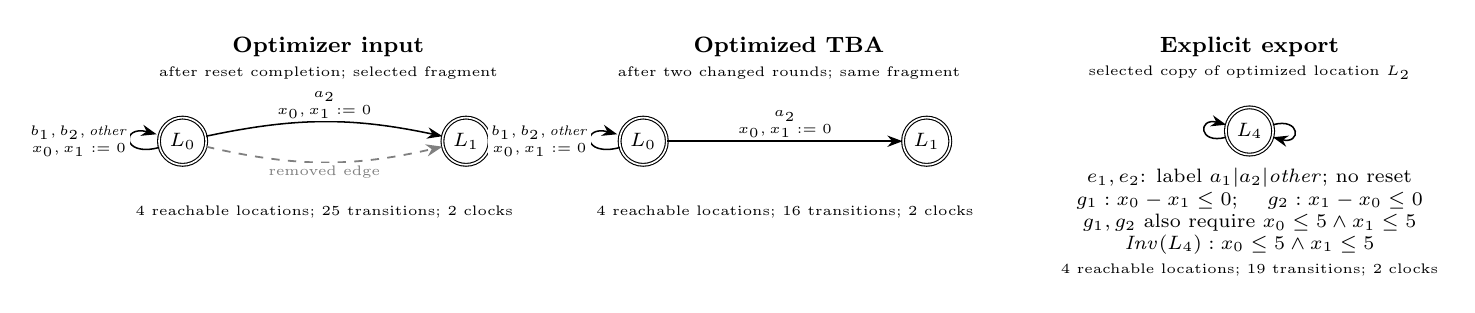
\begin{tikzpicture}[
  state/.style={circle,double,draw,minimum size=6mm,inner sep=1pt,font=\scriptsize},
  edge/.style={->,>=Stealth,line width=0.55pt},
  removed/.style={->,>=Stealth,dashed,gray,line width=0.65pt},
  lab/.style={font=\tiny,align=center,fill=white,inner sep=1pt},
  title/.style={font=\footnotesize\bfseries,align=center},
  small/.style={font=\tiny,align=center},
  detail/.style={font=\scriptsize,align=center}
]
% Each panel is a selected subgraph of the corresponding saved full automaton.
\begin{scope}[xshift=0cm]
  \node[title] at (2.6,2.05) {Optimizer input};
  \node[small] at (2.6,1.72) {after reset completion; selected fragment};
  \node[state] (i0) at (0.75,0.85) {$L_0$};
  \node[state] (i1) at (4.35,0.85) {$L_1$};
  \draw[edge] (i0) edge[loop left] node[lab,left]
    {$b_1,b_2,\mathit{other}$\\$x_0,x_1:=0$} (i0);
  \draw[edge] (i0) to[bend left=12] node[lab,above]
    {$a_2$\\$x_0,x_1:=0$} (i1);
  \draw[removed] (i0) to[bend right=13] node[lab,below]
    {removed edge} (i1);
  \node[small] at (2.55,-0.05)
    {$4$ reachable locations; $25$ transitions; $2$ clocks};
\end{scope}
\begin{scope}[xshift=5.85cm]
  \node[title] at (2.6,2.05) {Optimized TBA};
  \node[small] at (2.6,1.72) {after two changed rounds; same fragment};
  \node[state] (o0) at (0.75,0.85) {$L_0$};
  \node[state] (o1) at (4.35,0.85) {$L_1$};
  \draw[edge] (o0) edge[loop left] node[lab,left]
    {$b_1,b_2,\mathit{other}$\\$x_0,x_1:=0$} (o0);
  \draw[edge] (o0) -- node[lab,above]
    {$a_2$\\$x_0,x_1:=0$} (o1);
  \node[small] at (2.55,-0.05)
    {$4$ reachable locations; $16$ transitions; $2$ clocks};
\end{scope}
\begin{scope}[xshift=11.7cm]
  \node[title] at (2.6,2.05) {Explicit export};
  \node[small] at (2.6,1.72) {selected copy of optimized location $L_2$};
  \node[state] (e4) at (2.6,0.98) {$L_4$};
  % Separate the two loop arcs from their longer guard descriptions.
  \draw[edge] (e4) edge[loop left,looseness=6] (e4);
  \draw[edge] (e4) edge[loop right,looseness=6] (e4);
  \node[detail] at (2.6,0.39)
    {$e_1,e_2$: label $a_1|a_2|\mathit{other}$; no reset};
  \node[detail] at (2.6,0.10)
    {$g_1:x_0-x_1\leq0$; \quad $g_2:x_1-x_0\leq0$};
  \node[detail] at (2.6,-0.19)
    {$g_1,g_2$ also require $x_0\leq5\land x_1\leq5$};
  \node[detail] at (2.6,-0.46)
    {$\mathit{Inv}(L_4):x_0\leq5\land x_1\leq5$};
  \node[small] at (2.6,-0.78)
    {$4$ reachable locations; $19$ transitions; $2$ clocks};
\end{scope}
\end{tikzpicture}

\caption{Selected subgraphs from the actual generated R2 files. The dashed input edge is absent after optimization; only one of the nine removed transitions is shown. The first two panels show a retained edge and loop. The export panel follows the optimized $L_2$ loop to its $L_4$ copy, where one source loop becomes two conjunctive-guard loops. The annotations list their diagonal atoms, shared unary bounds, and invariant. Counts below summarize the complete automata: reachable locations, transitions, and active clocks. The internal output-shape guarantee is proved in Rocq; the displayed graph and counts are measurements.}
\label{fig:R2-generated}
\end{figure*}

The export continues by splitting disjunctive guards into conjunctive transitions, normalizing, pruning unreachable copies, and merging the initial location when an equivalent copy exists. A final symbolic pass groups transitions with the same source, target, and resets and stores their labels as Boolean conditions for drawings.

\subsection{Whole-export preservation and output shape}
\begin{theorem}[Export preservation]
\label{thm:export}
For every invariant-free TBA provided to the verified export interface, the explicit export preserves its timed-word language. The resulting automaton has conjunctive transition guards and conjunctive location invariants.
\end{theorem}
\begin{proof}
The explicit construction composes verified transition merging, invariant splitting, guard splitting, normalization, pruning, and initial-location merging; its timed-word preservation result is \texttt{export\_accepts}. The output shape is established by \texttt{export\_guards\_conjunctive} and \texttt{export\_invariants\_conjunctive}. A separate symbolic grouping pass preserves timed-word acceptance by \texttt{symbolic\_accepts} (with the extended-word result \texttt{symbolic\_ext\_accepts}).
\end{proof}
For reuse with another producer or checker, the theorem's output contract is
summarized in Table~\ref{tab:export-contract}.
\begin{table*}[t]
\centering
\caption{Contract of the verified optimization and export pipeline. The
explicit and symbolic outputs preserve the timed-word language of the TBA
provided to the Rocq interface.}
\label{tab:export-contract}
\small
\begin{tabular}{@{}p{0.22\textwidth}p{0.70\textwidth}@{}}
\toprule
Aspect & Guaranteed result\\
\midrule
Timed-word language & Preserved by every optimization round and by complete export under the development's existential initial-clock semantics.\\
Explicit guards & Conjunctions of event literals and clock comparisons; export may introduce clock-difference comparisons in entry conditions.\\
Location invariants & Conjunctions of non-strict clock upper bounds.\\
Symbolic output & Groups transitions with the same source, target, and reset set under Boolean labels; the symbolic automaton also preserves acceptance.\\
Input adapter & A third-party parser or conversion into the Rocq TBA representation requires a separate correspondence proof to join the verified boundary.\\
\bottomrule
\end{tabular}
\end{table*}
The theorem holds for every TBA of the formula-indexed clock interface: it requires no MTL provenance,
determinism, or particular upstream producer.

The saved generated files for the R2 input, optimized automaton, and export
are provided in \path{evaluation/generated\_examples/R2/}. Their run
metadata and the distinction between this current snapshot and the preserved
five-run medians are recorded alongside the files. This example shows an
actual optimizer/export interaction, while the separate synthetic ablation
in Section~\ref{sec:evaluation} isolates pass effects on direct TBA records.

\section{Composition with the MTL-to-TBA Correctness Theorem}
\label{sec:composition}
The earlier article~\cite{fares_bodeveix_mtl_translation} proves that its specified compiler preserves the
timed-word semantics of every applicable formula, provided the propositional
B\"uchi backend satisfies its stated language contract. The results of this
paper then preserve the language of the resulting TBA through any finite
number of optimization rounds and through export. The repository already
proves the composition as \texttt{MTL\_to\_exported\_correct\_with}; its
statement is
\begin{theorem}[End-to-end composition]
\label{thm:composition}
For every $n\in\Nat$, formula $f$, backend automaton $A$ and timed word $w$,
\[
\begin{gathered}
  \Bigl(\forall s:\mathsf{pword}(f),\Bigr.\\
  \Bigl.\mathsf{PBA\_accepts}(A,s)\leftrightarrow
       \mathsf{psat}(s,0,\T(f))\Bigr)\ \land\ \mathsf{well\_formed}(f)
  \\
  \Longrightarrow\quad
  \mathsf{msat}(w,0,f)\ \leftrightarrow\
  \mathsf{DTA\_accepts}(D_n,w),
  \\
  \begin{aligned}
  D_n &= \export(\\
        &\qquad\optimize(n,\mathsf{compile\_with}(A))).
  \end{aligned}
\end{gathered}
\]
\end{theorem}
\begin{proof}
The translation theorem
\path{MTL_to_TBA_correct_with}
gives the first equivalence below. The other two are the preservation results of
this paper, which do not depend on how $C$ was produced. Let $C=\mathsf{compile\_with}(A)$,
$O_n=\optimize(n,C)$, and $D_n=\export(O_n)$. Then
\[
\begin{aligned}
\mathsf{msat}(w,0,f) &\leftrightarrow \mathsf{TBA\_accepts}(C,w)\\
\mathsf{TBA\_accepts}(C,w) &\leftrightarrow \mathsf{TBA\_accepts}(O_n,w)\\
\mathsf{TBA\_accepts}(O_n,w) &\leftrightarrow \mathsf{DTA\_accepts}(D_n,w).
\end{aligned}
\]
The repository theorem
\path{MTL_to_exported_correct_with}
performs this composition. This paper adds no proof of the MTL translation.
\end{proof}
The first hypothesis is exactly the backend contract of
\path{MTL_to_TBA_correct_with}, required on the action-consistent
propositional words (those in which the negated action atom is the complement
of the action atom); \texttt{well\_formed} requires
nonnegative non-strict upper bounds and strictly positive bounds for the
other primitive timed operators. No convergence premise is imposed on
$n$: \path{optimize_accepts} proves preservation by induction for every
finite round count, and \path{export_accepts} then preserves the optimized
TBA's language. The implementation's 50-round stop is a practical driver
policy, not part of this theorem.

The theorem's conclusion concerns the internal exported DTA record and the
development's existential initial-clock semantics. It does not establish
Spot's correctness unless the backend premise is separately discharged, nor
does it prove correctness of the LBTT importer, XML printer, XML parser, or
UPPAAL execution. A second mechanized theorem,
\path{MTL_to_exported_correct0_with}, derives the corresponding
zero-initialized result when
$\texttt{init\_free}(\export(\optimize(n,\mathsf{compile\_with}(A))))=\texttt{true}$.
The underlying lemma \path{init_free_accepts0} holds for every exported
automaton on which the check succeeds; nothing guarantees that the check
succeeds on an automaton whose acceptance relies on nonzero initial clock values.

The separately verified all-copy policy yields the parallel theorem
\path{MTL_to_exported_all_correct_with}. For the same $n$, $f$,
$A$, and $w$, under the same backend contract and
$\mathsf{well\_formed}(f)$ hypothesis, it proves
\[
\begin{aligned}
\mathsf{msat}(w,0,f)
&\leftrightarrow
\mathsf{DTA\_accepts}(\export_{\mathrm{all}}(B),w),\\
B&=\optimize(n,\mathsf{compile\_with}(A)).
\end{aligned}
\]
Its conclusion has the same internal-DTA and existential-initial-clock
boundary. The all-copy theorem does not strengthen the zero-initialization
claim or verify XML serialization.

\section{Tool Architecture and Use in UPPAAL}
\label{sec:toolchain}
\subsection{Implementation and proof boundary}
The OCaml module \texttt{optim.ml} is extracted from Rocq and contains the
verified optimization and export functions. The integrated executable also
contains handwritten input, iteration, and output code. These adapters and
the XML/DOT printers are outside the transformation proofs. A converter from
an external automaton format must establish its own correspondence with the
Rocq TBA type. A clean Rocq 9.0.1 build, independent \texttt{coqchk} run,
and OCaml 5.4.0 rebuild are recorded in the accompanying artifact audit.
The UPPAAL 5.0.0 queries were rerun in this revision and agree with the
archived verdicts.

The project-wide axiom \path{LTL_TO_BUCHI_CORRECT} states the assumed
correctness of the upstream LTL-to-B\"uchi backend. Convenience theorem
variants use it when backend correctness is not an explicit argument. The
theorems \path{optimize_accepts}, \path{split_accepts}, and
\path{export_accepts} theorems quantify over arbitrary values of the
formal interface and do not use that project axiom. The theorem
\path{MTL_to_exported_correct_with} keeps the propositional-backend
equivalence as an explicit premise. Its fresh assumptions audit reports
standard classical Rocq library principles, including
\path{ClassicalDedekindReals.sig_forall_dec}, but no project-specific
backend axiom. The axiom \path{LTL_TO_BUCHI_CORRECT} appears in
convenience theorems that discharge that premise using the project axiom.
The artifact records the separate \texttt{Print Assumptions} results.

In the integrated workflow, the upstream producer supplies a TBA at the
optimizer boundary after its own construction stages. The earlier article~\cite{fares_bodeveix_mtl_translation} specifies and
proves the MTL-to-TBA translation; this paper takes that resulting TBA as an
input and concerns only the subsequent optimizer and exporter. The driver
iterates optimization until structural stability or a 50-round cap, then
applies export. This cap is an implementation policy; language preservation
holds for every finite round count.

The preservation theorems use existential initial clock values. UPPAAL starts clocks at zero. The verified \texttt{init\_free} check bridges the two conventions for every exported automaton on which it succeeds; when it fails, which can happen for an external automaton whose acceptance relies on nonzero initial clock values, no zero-initialization conclusion is drawn.

\subsection{Input contract for an external TBA}
\label{sec:generic-input}
The interface starts from a finite TBA value
$(L,\ell_0,X,E,\mathit{Acc})$ in the Rocq representation. Its clock set
$X$ is \path{Clock root}, the timed subformulas of a formula \path{root}
fixed by the development; an automaton with $k$ clocks is represented by
choosing any formula with at least $k$ distinct timed subformulas, which then
serve only as clock names. Its transitions carry
event conditions, finite conjunctions of unary clock comparisons, and reset
sets; the starting value has no location-invariant annotation. The invariant
synthesis pass derives that annotation from outgoing guards. The theorem
does not require a complete or deterministic transition relation, a particular
number of clocks, or a connection to a temporal-logic translator. A third-party
producer can therefore use the proved functions after converting its automaton
to this representation and naming its clocks in this way.

The conversion is a semantic boundary: it must retain the alphabet and the
meaning of each event condition, preserve which clocks are tested and reset,
and map accepting locations without changing their marking. The paper's
repository provides the Rocq type and extracted optimizer, but not a verified
reader for arbitrary third-party formats. Any such reader belongs to the
trusted interface until its correspondence with the Rocq value is proved. The
same applies to interpreting the result in a target checker: export proves
language preservation for the Rocq representation, while a separate bridge is
needed to identify the checker's parsed model with that value. This boundary
keeps the central optimization theorem independent of the producer while making the
work needed to reuse it explicit.

\subsection{Initialization interface}
The preservation theorems use existential initial clock values,
whereas UPPAAL initializes clocks to zero. The proved
\texttt{MTL\_to\_exported\_correct0\_with} theorem gives the zero-initialized
result for the formula-indexed workflow when the verified
\texttt{init\_free} check succeeds. All 29 completed benchmark outputs pass
that check; the two timed-out configurations produce no output to check. For
an external automaton the same check applies, and the zero-initialized
conclusion is available only when it succeeds.

\subsection{Using exported automata in UPPAAL}
The language-preservation theorem concerns infinite timed words with one
event at each position, strictly increasing timestamps, divergent time, and
the development's clock initialization semantics. A UPPAAL composition must
preserve the assumptions needed to interpret its traces in that model:
\begin{enumerate}[label=(C\arabic*),leftmargin=*]
  \item \emph{Events and time.} The system must synchronize each observable
        event with the property automaton, prevent zero-delay consecutive
        events (for example, reset a system clock $z$ on each emission and
        require $z>0$ on the next), and admit time-divergent infinite
        executions. Reachability alone does not rule out a Zeno continuation.
  \item \emph{Initial clocks.} UPPAAL initializes clocks to zero, while the
        preservation theorems use existential initial values. The
        zero-initialized conclusion requires the \texttt{init\_free} check
        of the preceding subsection to succeed on the exported automaton.
  \item \emph{Acceptance.} UPPAAL's ordinary reachability interface does not
        check B\"uchi acceptance. For safety, use a violation automaton with
        an accepting sink that is reached when a violation occurs and has a
        loop on every event. Liveness requires a B\"uchi emptiness checker
        that restricts attention to time-divergent runs; the artifact uses
        TChecker for this task.
  \item \emph{Time constraints in products.} Location invariants are part of
        the automaton semantics and can block time in a product, thereby
        removing system behaviors. An exported property automaton is not a
        passive observer unless its effect on the product is separately
        justified. Check deadlock or timelock conditions on the system as
        appropriate.
  \item \emph{Numbers.} The integrated tool accepts integer bounds in
        $[0,2^{30}]$. The Rocq theorems are over real-valued clocks; the
        extracted implementation's arithmetic and the UPPAAL printer are
        covered only on the tool's restricted numeric domain.
\end{enumerate}

The generated XML has a \texttt{Property} template for the automaton and an
\texttt{Env} template that can emit events for standalone language
exploration. In a system check, the system replaces \texttt{Env} and
synchronizes its observable events with \texttt{Property}; the event
\texttt{other} denotes any event outside the finite set named in the formula.
Accepting locations are named \texttt{A}$n$ in the output, but those names do
not make UPPAAL check B\"uchi acceptance. For a safety requirement, the
reachability query must use an automaton for its violations with a sink entered
once the violation has occurred. For a liveness requirement, reachability of
such a sink is not the right check and an emptiness procedure for
time-divergent B\"uchi runs is needed.

For a safety property $\varphi$, let $\mathcal A_{\neg\varphi}$ be a
violation automaton whose accepting sink has no invariant and loops on every
event. Compose it with a system $S$ that synchronizes the same event alphabet
and can extend every queried prefix to a time-divergent execution. Under
(C1)--(C3) and the appropriate initialization condition in (C2), the query
\texttt{E<> P.A} detects a system behavior violating $\varphi$ when the
automaton recognizes exactly those violations. This query-level equivalence
is an argument about the chosen system and automaton; it is not proved by the
Rocq optimization or export theorem. The case-study models below
report the model checks and diagnostic traces for the four packaged systems.

\subsection{Availability}
This project contains proof sources, extracted implementation, benchmark tables and raw data, reproduction scripts, and UPPAAL case-study models, together with the LaTeX source and build instructions. The invariant, optimization, and export formalization files contain the generic pass results; their theorem names are listed in Table~\ref{tab:post-passes}. The project repository is at \url{https://github.com/efares1/rocq-tba-optimization-uppaal-export}, and the repository of the translation article is at \url{https://github.com/efares1/rocq-mtl-to-tba-translation}. The revisions described here are the releases tagged \texttt{v1.1} in both repositories.

\subsection{Build and artifact layout}
The verified functions are defined under \texttt{proof/} and extracted into
\texttt{tool/src/optim.ml}. The project Makefile compiles the Rocq
development and extracts the executable functions. Hand-written components
include the parser, Spot invocation, LBTT reader, iteration driver, and
XML/DOT printers; the script that removes unreachable extracted definitions
and the Rocq/OCaml toolchains are also part of the implementation's trusted
base. The repository includes the machine record, raw benchmark runs, TSV
summaries, table generator, formulas, UPPAAL models and queries, and
reproduction instructions in \texttt{README.md}.

Table~\ref{tab:component-boundary} separates the verified transformations
from the interfaces that connect them to the surrounding tools.
\begin{table*}[t]
\centering
\caption{Runtime stages and their proof boundary. The preservation theorems begin
with a TBA in the Rocq representation; the Spot-based formula front end is one
client of the verified optimizer and exporter.}
\label{tab:component-boundary}
\footnotesize
\begin{tabular}{@{}p{0.22\textwidth}p{0.35\textwidth}p{0.35\textwidth}@{}}
\toprule
Stage & Implementation & Guarantee or boundary\\
\midrule
TBA input and adapter & Rocq TBA value or a parser/converter supplied by the caller & Pass results start at this representation; an external adapter is outside the theorem unless separately verified.\\
Spot-based front end & Spot call and hand-written LBTT reader in \texttt{mtl2tba} & Used by the integrated formula workflow; outside the TBA preservation theorems.\\
Optimization rounds & Extracted from \texttt{MTL\_to\_TBA\_Optimizations.v} & \texttt{optimize\_accepts}, for every TBA and every round count.\\
Iteration driver & Hand-written OCaml structural comparison; stops at equality or 50 rounds & The proof does not assume convergence or a particular stopping point.\\
UPPAAL export & Extracted from \texttt{MTL\_to\_TBA\_Export.v} & \texttt{export\_accepts} and conjunctive guard/invariant results.\\
Symbolic grouping & Extracted from \texttt{MTL\_to\_TBA\_Symbolic.v} & \texttt{symbolic\_ext\_accepts}.\\
XML, DOT, and PDF output & Hand-written printers and Graphviz & Outside the Rocq language-preservation results.\\
Numeric realization & OCaml floating point with integer bounds in $[0,2^{30}]$ & Exactness follows from inspection of the extracted operations, not a mechanized theorem.\\
\bottomrule
\end{tabular}
\end{table*}

In the extracted code, structural equality decides formula and clock
identity, and Boolean checks implement conditions whose soundness is proved
in Rocq. Real comparisons are realized by OCaml floating-point operations.
Input constants lie in $[0,2^{30}]$; the inspected operations produce only
such constants, their differences, or their negations. These values are
exactly representable by the 53-bit significand of a double, and the printed
constants fit UPPAAL's 32-bit integer domain. This arithmetic argument is
based on inspection of the extracted implementation rather than a theorem
about OCaml or the printer. Rational constants can be handled by a common time
scaling only when every scaled bound remains an integer in $[0,2^{30}]$; timing
constants in any surrounding system model must be scaled by the same factor.

\section{Evaluation}
\label{sec:evaluation}
\subsection{Questions, evidence, and setup}
The evaluation asks four separate questions. First, which structures do the
verified optimization passes remove or simplify? Second, what size and timing
cost does conversion to conjunctive guards and invariants add? Third, do the
packaged system checks behave as intended? Fourth, does optimization affect a
matched downstream check? Internal output shape is a Rocq theorem; external
checker verdicts and resource use are experimental evidence. The matched
TChecker cases below show unchanged exploration on systems whose exported
models are byte-identical before and after optimization; they do not establish
a general cost improvement.

We retain the 31-attempt F/R/N benchmark as an upstream-generated
group. The optimizer input is the automaton after reset completion, shown as
Comp. in Table~\ref{tab:optimizer-benchmarks}. Of the 31 attempted
configurations, 29 completed this upstream stage and supplied an optimizer
input; R7 and R8 timed out before the measured boundary. Formula rewriting, Spot
configuration, cube expansion, relaxation, and reset completion happen
upstream; their effects are not credited to the optimizer. The runs use the
tool's default front end, which before translation rewrites
$\Box\Diamond_{\ge d}\varphi$ into $\Box\Diamond\varphi$ and
$\Diamond\Box_{\ge d}\varphi$ into $\Diamond\Box\varphi$, and which replaces
the Until of the clauses of upper-bounded hatted Until by a weak Until. The
end-to-end theorem for this front end is
\path{MTL_to_exported_correct0_recur_weak_with}
(\path{MTL_to_TBA_Recur.v}); the optimizer theorems are unaffected, since
they hold for every input TBA of the interface. Results
come from the repository's five-run medians on Ubuntu 26.04/WSL 2, an Intel
Core i7-8650U at 1.9 GHz with 11.7 GB memory, OCaml 5.4.0, Rocq 9.0.1, and
Spot 2.16. The fresh run used five repetitions per completed configuration
and a 300-second limit per attempt. Its run log, machine record, summary
table, and generated automata are preserved under
\path{evaluation/runs/2026-10-12-full-eval-v2/}.
\begin{table*}[t]
\centering
\caption{Fresh five-run post-processing measurements (12 October 2026) for 31 attempted upstream-generated configurations; 29 produced optimizer inputs. Comp. is the automaton after reset completion. $L$ counts graph-reachable locations, $E$ counts transitions from those locations, and $C$ counts active clocks used in guards or resets; $n_f$ is the formula-clock-key count. Opt. and Exp. give reachable $L/E/C$, changed optimization rounds, stage medians, invariant-bearing locations, and diagonal-guard occurrences. R7 and R8 time out upstream, before the optimizer boundary.}
\label{tab:optimizer-benchmarks}
\scriptsize
\setlength{\tabcolsep}{3pt}
\begin{tabular}{@{}lccccccccc@{}}
\toprule
ID & Comp. $L/E/C$ & $n_f$ & Opt. $L/E/C$ & Rnds & Opt. (s) & Exp. $L/E/C$ & Inv. & Diag. & Exp. (s)\\
\midrule
F1 & 2/5/1 & 1 & 2/5/1 & 1 & $<0.01$ & 2/5/1 & 1 & 0 & $<0.01$\\
F2 & 2/5/1 & 1 & 1/1/0 & 1 & $<0.01$ & 1/1/0 & 0 & 0 & $<0.01$\\
F3 & 2/5/1 & 1 & 2/5/1 & 1 & $<0.01$ & 2/5/1 & 0 & 0 & $<0.01$\\
F3b & 1/1/0 & 1 & 1/1/0 & 0 & $<0.01$ & 1/1/0 & 0 & 0 & $<0.01$\\
F4 & 2/5/1 & 1 & 2/5/1 & 1 & $<0.01$ & 2/5/1 & 1 & 0 & $<0.01$\\
F5 & 7/38/1 & 1 & 7/25/1 & 1 & $<0.01$ & 7/25/1 & 0 & 0 & 0.01\\
F6 & 7/38/1 & 1 & 7/25/1 & 1 & $<0.01$ & 7/25/1 & 0 & 0 & $<0.01$\\
F7 & 2/4/1 & 1 & 2/4/1 & 1 & $<0.01$ & 2/4/1 & 1 & 0 & $<0.01$\\
F8 & 2/4/0 & 0 & 2/4/0 & 1 & $<0.01$ & 2/4/0 & 0 & 0 & $<0.01$\\
F9 & 4/9/2 & 2 & 4/9/2 & 1 & $<0.01$ & 4/9/2 & 2 & 0 & $<0.01$\\
F10 & 5/13/3 & 3 & 5/13/3 & 1 & $<0.01$ & 5/13/3 & 2 & 0 & $<0.01$\\
F11 & 4/7/2 & 2 & 3/4/1 & 2 & $<0.01$ & 3/4/1 & 1 & 0 & $<0.01$\\
F12 & 3/9/2 & 2 & 2/5/2 & 2 & $<0.01$ & 2/5/2 & 1 & 0 & $<0.01$\\
F13 & 3/6/2 & 2 & 2/3/1 & 2 & $<0.01$ & 2/3/1 & 1 & 0 & $<0.01$\\
F14 & 6/23/2 & 2 & 6/17/2 & 1 & $<0.01$ & 6/19/2 & 4 & 2 & $<0.01$\\
R1 & 2/5/1 & 1 & 2/5/1 & 1 & $<0.01$ & 2/5/1 & 1 & 0 & $<0.01$\\
R2 & 4/25/2 & 2 & 4/16/2 & 2 & $<0.01$ & 4/19/2 & 3 & 2 & $<0.01$\\
R3 & 8/125/3 & 3 & 8/44/3 & 3 & 0.01 & 8/67/3 & 7 & 30 & 0.01\\
R4 & 16/625/4 & 4 & 16/112/4 & 4 & 0.06 & 16/217/4 & 15 & 192 & 0.16\\
R5 & 32/3125/5 & 5 & 32/272/5 & 5 & 0.94 & 32/651/5 & 31 & 880 & 1.45\\
R6 & 64/15625/6 & 6 & 64/640/6 & 6 & 17.81 & 64/1837/6 & 63 & 3360 & 10.67\\
R7 & -- & -- & -- & -- & -- & -- & -- & -- & --\\
R8 & -- & -- & -- & -- & -- & -- & -- & -- & --\\
N1 & 3/5/1 & 1 & 3/5/1 & 1 & $<0.01$ & 3/5/1 & 1 & 0 & $<0.01$\\
N2 & 4/11/2 & 2 & 4/9/2 & 1 & $<0.01$ & 4/9/2 & 2 & 0 & $<0.01$\\
N3 & 5/21/3 & 3 & 5/16/3 & 1 & $<0.01$ & 5/16/3 & 3 & 0 & $<0.01$\\
N4 & 6/36/4 & 4 & 6/25/4 & 1 & $<0.01$ & 6/25/4 & 4 & 0 & 0.01\\
N5 & 7/57/5 & 5 & 7/36/5 & 1 & 0.01 & 7/36/5 & 5 & 0 & 0.02\\
N6 & 8/85/6 & 6 & 8/49/6 & 1 & 0.03 & 8/49/6 & 6 & 0 & 0.06\\
N7 & 9/121/7 & 7 & 9/64/7 & 1 & 0.10 & 9/64/7 & 7 & 0 & 0.23\\
N8 & 10/166/8 & 8 & 10/81/8 & 1 & 0.33 & 10/81/8 & 8 & 0 & 0.70\\
\bottomrule
\end{tabular}
\end{table*}


Across the 29 completed inputs, the sum of reachable transition counts falls
from 20,204 at the post-reset-completion boundary to 1,510 after optimization
(an aggregate reduction of 92.53\%). Sixteen cases have fewer transitions
and 13 are unchanged. This aggregate is strongly skewed: R6 contributes
14,985 of the 18,694 removed transitions, so the percentage is not a typical
per-instance reduction. Active clocks used in guards or resets sum from 77
to 74; only three cases (F2, F11, F13) reduce this count. The export stage has a different
effect: explicit transitions sum from 1,510 to 3,219, an increase of
113.18\%; six exports grow and 23 have the same count as their optimized
input. Export-size change is reported separately from optimization and is
not counted as an optimization regression.
\begin{table*}[t]
\centering
\caption{Family aggregates derived from the completed rows of Table~\ref{tab:optimizer-benchmarks}. Edge totals are measured at the post-reset-completion optimizer boundary, after optimization, and after explicit export.}
\label{tab:optimizer-aggregates}
\scriptsize
\setlength{\tabcolsep}{3pt}
\begin{tabular}{@{}p{0.22\textwidth}rrrrrr@{}}
\toprule
Group & $n$ & Input $\sum E$ & Opt. $\sum E$ & Reduction & Exp. $\sum E$ & Cases $\downarrow/= /\uparrow$\\
\midrule
F group & 15 & 198 & 138 & 30.30\% & 140 & 7/8/0 \\
bounded-response R group & 6 & 19,530 & 1,089 & 94.42\% & 2,796 & 5/1/0 \\
N group & 8 & 502 & 285 & 43.23\% & 285 & 7/1/0 \\
\bottomrule
\end{tabular}
\end{table*}

The family breakdown shows how concentrated these totals are. The six
completed bounded-response R cases account for 18,441 of the 18,694 removed
transitions (98.65\%); the F and N groups remove 36 and 217, respectively.
The R group's explicit export grows from 1,089 to 2,796 transitions, while
the F group grows by two and the N group is unchanged. Thus the aggregate
optimizer reduction is driven mainly by one bounded-response family, and the
export expansion is a separate representation cost concentrated in that same
family.

Part of this reduction only re-merges the cubes that Spot emits one by one.
With symbolic grouping applied in both runs, the optimizer alone lowers the
symbolic transition count (\texttt{-n 0} against the default) from 704 to 354
(50\%) on the 27 configurations whose unoptimized export completes: from 364
to 226 on F and N, and from 340 to 128 on R1--R4. It is smaller in 14 and
equal in 13 (supplement). The unoptimized export of R5 and R6 does not finish
within 300 s, whereas the optimized pipeline completes them in 2.3 s and 33.7 s.

\begin{figure*}[t]
\centering
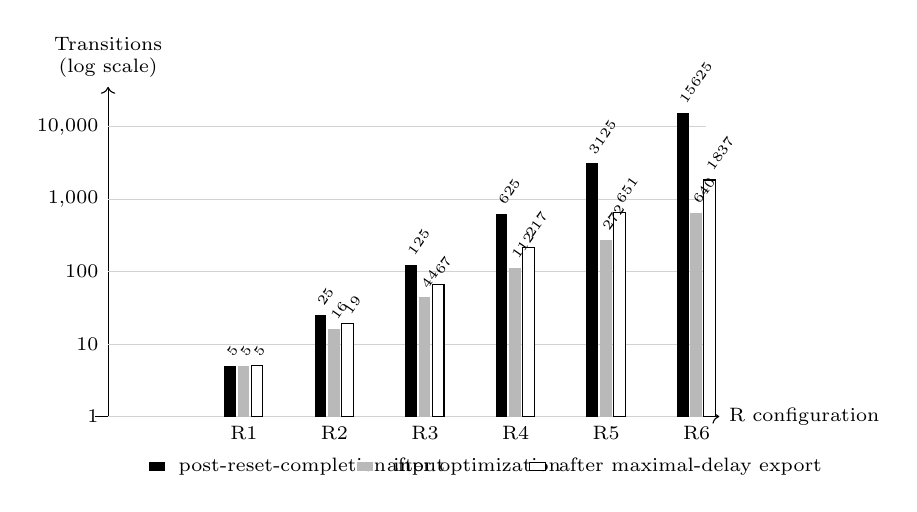
\begin{tikzpicture}[x=1.15cm,y=0.92cm,font=\scriptsize]
  % Vertical positions encode log10(edge count); the labelled y ticks are
  % 1, 10, 100, 1,000, and 10,000 transitions.
  \draw[->] (0.1,0) -- (7.0,0) node[right] {R configuration};
  \draw[->] (0.25,0) -- (0.25,4.55) node[above,align=center]
    {Transitions\\(log scale)};
  \foreach \y/\lab in {0/1,1/10,2/100,3/1{,}000,4/10{,}000} {
    \draw[gray!35] (0.25,\y) -- (6.85,\y);
    \node[left] at (0.25,\y) {\lab};
  }
  % Bars use log10(value) as height. Values above bars are exact counts.
  \foreach \x/\vin/\hin/\vopt/\hopt/\vexp/\hexp in {
    1/5/0.699/5/0.699/5/0.699,
    2/25/1.398/16/1.204/19/1.279,
    3/125/2.097/44/1.643/67/1.826,
    4/625/2.796/112/2.049/217/2.336,
    5/3125/3.494/272/2.435/651/2.814,
    6/15625/4.194/640/2.806/1837/3.264
  } {
    \pgfmathsetmacro{\xc}{\x+0.75}
    \pgfmathsetmacro{\xa}{\xc-0.22}
    \pgfmathsetmacro{\xb}{\xc-0.07}
    \pgfmathsetmacro{\xd}{\xc+0.08}
    \fill[black] (\xa,0) rectangle +(0.13,\hin);
    \fill[gray!55] (\xb,0) rectangle +(0.13,\hopt);
    \fill[white] (\xd,0) rectangle +(0.13,\hexp);
    \draw (\xd,0) rectangle +(0.13,\hexp);
    \node[rotate=55,anchor=west,font=\tiny] at (\xa,\hin+0.04) {\vin};
    \node[rotate=55,anchor=west,font=\tiny] at (\xb,\hopt+0.04) {\vopt};
    \node[rotate=55,anchor=west,font=\tiny] at (\xd,\hexp+0.04) {\vexp};
    \node[below] at (\xc,0) {R\x};
  }
  \fill[black] (0.7,-0.75) rectangle +(0.18,0.12);
  \node[right] at (0.92,-0.69) {post-reset-completion input};
  \fill[gray!55] (3.0,-0.75) rectangle +(0.18,0.12);
  \node[right] at (3.22,-0.69) {after optimization};
  \fill[white] (4.9,-0.75) rectangle +(0.18,0.12);
  \draw (4.9,-0.75) rectangle +(0.18,0.12);
  \node[right] at (5.12,-0.69) {after maximal-delay export};
\end{tikzpicture}

\caption{Post-reset-completion input, optimized TBA, and maximal-delay
explicit export for R1--R6. The logarithmic vertical axis makes the R6
concentration visible. These are the fresh five-run-median structural
counts; Comp. is the optimizer boundary, regardless of whether an upstream
Spot count happens to match it.}
\label{fig:R-transition-counts}
\end{figure*}

\subsection{Optimization effects on the generated group}
In R6, Spot emits 64 states and 15,625 cube-split transitions. The recorded
post-reset-completion optimizer input also has 64 locations and 15,625
transitions; the equality of these two edge counts is specific to R6, and the
Comp. column is the authoritative optimizer boundary. Six optimization
rounds reduce the transition relation to 640 edges and retain six clocks.
Export then produces 1,837 explicit edges, 63 invariant-bearing locations,
and 3,360 clock-difference guard occurrences; symbolic grouping represents
the output with 448 transitions. The larger explicit edge count results from
splitting disjunctive guards and adding entry conditions for invariant copies.
It measures the cost of the target representation, not a reversal of the
optimizer's reduction. In the fresh run, median optimizer and export times
are 19.812 s and 12.481 s, respectively. The October 10 and October 7 runs reported
19.345 and 13.410 s, and 25.091 and 14.572 s, with the same structural
counts; no cause for the timing changes is assigned. The generated-group table separately reports the
stage after reset completion so that upstream processing is not folded into
these optimizer measurements.

The same distinction matters for the other generated inputs. For example,
F11 starts from its actual four-location, seven-transition, two-clock TBA
after reset completion; two rounds leave the four locations and seven
transitions and remove one clock. The two locations that correspond to
states 2 and 3 of the earlier article's worked example stay separate: one
could be dropped, because $x\ge2$ always holds in the second, but location
merging requires twin transitions and their guards differ
($x\ge2\land x\le5$ against $x\le5$). N8 spends most of its end-to-end time in Spot,
whereas its recorded optimizer and exporter stages take 0.26 s and 0.68 s.
These cases show that the optimizer's cost depends on its input relation and
that the upstream producer can dominate total tool time. They do not support
a general runtime or size bound. With the tool's \texttt{-spot-level low}
option (default unchanged), N8 takes 8.9 s instead of 101.6 s, and the total
over the 29 completed configurations falls from 163 s to 46 s (one run
against the five-run medians); optimized sizes are identical except for F5
and F6 (25 to 27 symbolic transitions). R6 is dominated by the optimizer and
the export, and its faster run (32.1 s against 46.8 s) is not attributed to
the level.

\subsection{External output-size reference}
CASAAL~\cite{casaal_tool} implements the MTL$_{0,\infty}$ construction of
Li et al.~\cite{li_spin7} and prints automata with Boolean transition labels.
It is not an interchangeable optimizer: it builds its automata by its own
construction, so its sizes are a reference for the final output, not a
baseline for the optimization passes. We ran it with mutually exclusive
events, which matches the one-event-per-position words of our semantics, and
compare reachable locations and symbolic transitions of our optimized output
with CASAAL's output on the 27 configurations that both tools completed and
that CASAAL encodes exactly. The counts coincide in 24 cases. For F5 and F6
our output is larger (7 locations and 25 symbolic transitions against 4 and
15); for F14 it is smaller (6 and 14 against 8 and 18). Clock counts coincide
except for F11, where two optimization rounds reduce the two clocks of the
post-reset-completion input to one while CASAAL uses two, and F8, where the
difference comes from the upstream rewriting of $\Box\Diamond_{\ge2}p$ into
$\Box\Diamond p$ and is not credited to the optimizer. In R6 both outputs
have 64 locations and 448 symbolic transitions, whereas the optimizer input
has 15,625 explicit transitions. Whether the two tools accept the same timed
words is a question about the translation, examined in the earlier
article~\cite{fares_bodeveix_mtl_translation}; this comparison concerns sizes only.

\subsection{Matched comparison of the two export policies}
We reran R2--R6 once with each verified split policy while holding the
optimized automaton fixed. For every formula, the optimized TBA DOT files
were byte-identical across the two invocations. The table reports the
explicit-edge counts, diagonal guard atoms, and single-run exporter time
returned by the tool. Across these five inputs, all-copy export has no
explicit-edge growth beyond the optimized relation and adds no diagonal
guards. Maximal-delay export adds explicit edges in each case and introduces
2--3,360 diagonal guard atoms. This is a measured property of this benchmark
family, not a general size theorem.

\begin{table*}[t]
\centering
\caption{Matched maximal-delay and all-copy exports for R2--R6. The two
policies receive byte-identical optimized TBA graphs. Export time is one
observed run per row and policy; it is descriptive and should not be read as
a stable speed ranking.}
\label{tab:generated-export-policy}
\scriptsize
\setlength{\tabcolsep}{4pt}
\begin{tabular}{@{}lrrrrrrr@{}}
\toprule
ID & Optimized $E$ & Max-delay $E$ & All-copy $E$ & Max-delay diagonal atoms & All-copy diagonal atoms & Max-delay time (s) & All-copy time (s)\\
\midrule
R2 & 16 & 19 & 16 & 2 & 0 & 0.002 & 0.005\\
R3 & 44 & 67 & 44 & 30 & 0 & 0.014 & 0.024\\
R4 & 112 & 217 & 112 & 192 & 0 & 0.195 & 0.190\\
R5 & 272 & 651 & 272 & 880 & 0 & 1.319 & 1.052\\
R6 & 640 & 1,837 & 640 & 3,360 & 0 & 9.689 & 9.614\\
\bottomrule
\end{tabular}
\end{table*}

Both policies retain the same reachable location counts, active clock counts,
and invariant-bearing locations on these runs. Peak RSS was measured for
each full tool process, including Spot and optimization: 17.2/17.3 MB for R2
and 108.5/107.0 MB for R6 (maximal-delay/all-copy). These process-level
measurements do not isolate export memory. The observed exporter times also
have no consistent ordering: all-copy takes longer for R2/R3 and shorter for
R4/R5, with similar times for R6. The R6 policy comparison uses the same
15,625-edge post-reset-completion input and six-round, 640-edge optimized
TBA; the upstream Spot count is context, not the optimizer's pre-state.

\subsection{Translator-independent synthetic TBA suite}
To exercise the interface without the MTL translator, we construct
16 small synthetic automata directly as Rocq-representation TBA records in
\path{evaluation/synthetic_tba_bench.ml}. Their clocks are named by the six
timed subformulas of a fixed formula, the conjunction of six hatted primitive
formulas over three events; this formula is never translated and serves only
as a supply of six clock names. Locations, event labels, unary guards,
resets, and accepting locations are written by hand for each record. The suite is explicitly
synthetic: it does not parse a third-party format and is not evidence of
industrial-model performance. Its records cover redundant guards,
contradictory guards, unsatisfiable labels, a source with no incoming edge,
dead resets, synchronously reset clocks, duplicate transitions, equivalent
locations, a disjunctive-invariant export, a stable no-change input, and
targeted backward/forward propagation and pass-interaction cases.
\begin{table*}[t]
\centering
\caption{Sixteen translator-independent synthetic TBA records. Count tuples are declared locations / transitions / distinct clocks / reset occurrences / unary guard atoms; the export tuple adds diagonal guard atoms. The $I$ field gives nonempty invariant locations:bound atoms. Optimization and export times are per-call means over 200 repeated in-memory runs; RSS is the peak for a separate single-model process. Full per-pass and reachability data are supplied in the artifact.}
\label{tab:synthetic-tba}
\scriptsize
\begin{tabular}{@{}lrrrrrrr@{}}
\toprule
Model & Input & Optimized & Rounds & Opt. (ms) & RSS (KiB) & Export & Exp. (ms)\\
\midrule
stable & 1/1/0/0/0 & 1/1/0/0/0; $I=0:0$ & 0 & 0.008 & 6364 & 2/1/0/0/0/0; $I=1:0$ & 0.089\\
redundant\_guard & 2/2/1/1/3 & 2/2/1/1/2; $I=2:2$ & 1 & 0.133 & 6460 & 4/2/1/1/2/0; $I=2:2$ & 0.197\\
contradictory\_guard & 2/2/1/0/2 & 2/1/0/0/0; $I=0:0$ & 1 & 0.042 & 6428 & 4/1/0/0/0/0; $I=1:0$ & 0.073\\
unsatisfiable\_label & 2/2/0/0/0 & 2/1/0/0/0; $I=0:0$ & 1 & 0.026 & 6352 & 4/1/0/0/0/0; $I=1:0$ & 0.143\\
isolated\_source & 3/2/0/0/0 & 3/1/0/0/0; $I=0:0$ & 1 & 0.027 & 6340 & 6/1/0/0/0/0; $I=1:0$ & 0.264\\
dead\_reset & 2/2/1/2/0 & 2/2/0/0/0; $I=0:0$ & 1 & 0.052 & 6468 & 4/2/0/0/0/0; $I=2:0$ & 0.150\\
normalization\_dead\_reset & 2/2/1/1/1 & 2/2/0/0/0; $I=0:0$ & 1 & 0.110 & 6336 & 4/2/0/0/0/0; $I=2:0$ & 0.491\\
synchronous\_clock\_merge & 2/3/2/2/2 & 2/3/1/1/2; $I=1:1$ & 2 & 0.673 & 6300 & 4/3/1/1/2/0; $I=2:1$ & 1.279\\
duplicate\_transition & 2/3/1/2/3 & 2/2/1/1/2; $I=2:2$ & 1 & 0.267 & 6364 & 4/2/1/1/2/0; $I=2:2$ & 0.478\\
equivalent\_locations & 3/4/0/0/0 & 3/2/0/0/0; $I=0:0$ & 2 & 0.104 & 6404 & 6/2/0/0/0/0; $I=2:0$ & 0.220\\
disjunctive\_invariant\_export & 3/3/2/0/2 & 3/3/2/0/2; $I=0:0$ & 0 & 0.095 & 6488 & 9/6/2/0/12/6; $I=3:2$ & 1.154\\
backward\_tightening & 2/2/1/0/2 & 2/2/1/0/2; $I=2:2$ & 1 & 0.093 & 6360 & 4/2/1/0/2/0; $I=2:2$ & 0.204\\
forward\_lower\_bound & 3/3/1/0/2 & 3/3/1/0/4; $I=2:2$ & 1 & 0.141 & 6460 & 6/3/1/0/4/0; $I=3:2$ & 0.654\\
forward\_contradiction\_cascade & 6/7/1/0/3 & 6/4/1/0/4; $I=1:1$ & 2 & 0.437 & 6428 & 12/4/1/0/4/0; $I=3:1$ & 1.082\\
backward\_contradiction\_cascade & 5/5/1/0/4 & 5/1/0/0/0; $I=0:0$ & 2 & 0.201 & 6320 & 10/1/0/0/0/0; $I=1:0$ & 0.180\\
clock\_merge\_contradiction\_cascade & 5/5/2/6/4 & 5/3/1/2/1; $I=1:1$ & 2 & 0.622 & 6484 & 10/2/1/2/1/0; $I=2:1$ & 0.598\\
\bottomrule
\end{tabular}
\end{table*}


The harness reports counts after every pass in every round and checks that
its profiled pass sequence is structurally equal to the extracted
\texttt{optimize\_step} on each round. It also times the unprofiled iterative
optimizer and export as means over 200 repeated in-memory calls per model.
Standalone process RSS ranges from 6,184 to 6,484 KiB. These short timings
and small, purpose-built records are microbenchmark evidence only; the raw
pass table and per-model RSS file are supplied for reproduction. Per-pass
times are recorded but are too small to support fine-grained speed rankings.

The targeted examples exercise both bound-propagation directions. Backward
synthesis tightens an incoming $x\leq5$ guard to $x\leq2$. Forward
propagation adds an entry lower bound $x\geq2$ to outgoing edges. In the
forward-cascade input, an alternate $x\leq10$ branch prevents backward
synthesis from creating the contradiction; forward propagation makes the
$x\leq1$ branch contradictory, and the following pruning stages remove its
unentered chain. Omitting forward propagation retains all seven input edges,
while the full optimizer leaves four. A separate backward cascade isolates
that pass. Table~\ref{tab:synthetic-interactions} shows input/output counts
and leave-one-operation-out effects.

The normalization/reset example removes a tautological $x\geq0$ guard before
dead-reset analysis, allowing its reset and active clock to be removed. The
synchronous-clock example first merges the clocks, then a later round detects
the conflicting $x\geq5\land x\leq3$ guard and prunes the branch. Other
records measure unsatisfiable-label elimination, no-incoming-source pruning,
transition subsumption, and equivalent-location merging. The no-incoming
operation is a local predecessor test, not full graph reachability. These
interactions explain the iterative design; preservation for each finite
iteration count follows from the proved pass composition.
\begin{table*}[t]
\centering
\caption{Measured direct TBA examples targeting propagation and pass interactions. Transition and clock counts are total records and active clocks. Leave-one-operation-out variants are experimental composites, not separately verified transformations.}
\label{tab:synthetic-interactions}
\scriptsize
\setlength{\tabcolsep}{3pt}
\begin{tabular}{@{}p{0.22\textwidth}cccp{0.39\textwidth}@{}}
\toprule
Case & Input $E/C$ & Full $E/C$ & Rounds & Measured target-pass effect when omitted\\
\midrule
Backward bound tightening & 2/1 & 2/1 & 1 & Incoming guard tightens from $x\leq5$ to $x\leq2$; omitting backward synthesis leaves $x\leq5$.\\
Forward lower-bound propagation & 3/1 & 3/1 & 1 & Entry fact $x\geq2$ is added to the outgoing $q$ edge; edge count is unchanged.\\
Forward contradiction cascade & 7/1 & 4/1 & 2 & Omitting forward propagation or contradiction removal retains 7 edges; the full run removes the $x\leq1$ branch and then prunes its unentered chain.\\
Backward contradiction cascade & 5/1 & 1/0 & 2 & Omitting backward synthesis leaves 2 edges/1 clock; omitting contradiction removal leaves 5/1.\\
Normalization and dead reset & 2/1 & 2/0 & 1 & Normalizing tautological $x\geq0$ enables reset removal; omitting either pass leaves 1 active clock.\\
Synchronous-clock contradiction & 5/2 & 3/1 & 2 & Merging the synchronously reset clocks exposes $x\geq5\land x\leq3$; omitting clock merge or contradiction removal leaves 5 edges/2 clocks.\\
\bottomrule
\end{tabular}
\end{table*}


Table~\ref{tab:synchronous-trace} gives the measured stage interaction for
the largest synchronously reset synthetic input. Unsatisfiable-label removal
first reduces the relation from seven edges to five. Dead-reset elimination
then lowers the active-clock count from six to four. The synchronous-clock
pass changes the synthesized invariant, and the next round's dead-reset pass
removes the remaining redundant resets, leaving one active clock. This is a
measurement of the extracted implementation; the language-preservation
claim follows separately from the proved pass composition.
\begin{table*}[t]
\centering
\caption{Measured trace for the six-clock synchronous-reset synthetic input. Counts are declared / reachable locations, transitions, active clocks, reset occurrences, guard atoms, invariant locations / atoms, and diagonal guard atoms. The export row is the internal explicit DTA.}
\label{tab:synchronous-trace}
\scriptsize
\setlength{\tabcolsep}{3pt}
\begin{tabular}{@{}p{0.27\textwidth}rrrrrrr@{}}
\toprule
Stage & $L/R$ & $E$ & $C$ & Resets & Guard atoms & Inv. $L/A$ & Diag.\\
\midrule
Input & 2/2 & 7 & 6 & 6 & 6 & 0/0 & 0 \\
R1: unsatisfiable-label removal & 2/2 & 5 & 6 & 6 & 4 & 0/0 & 0 \\
R1: dead-reset elimination & 2/2 & 5 & 4 & 4 & 4 & 0/0 & 0 \\
R1: synchronous-clock pass & 2/2 & 5 & 4 & 4 & 4 & 1/1 & 0 \\
R2: dead-reset elimination & 2/2 & 5 & 1 & 1 & 4 & 1/1 & 0 \\
Optimized fixed point & 2/2 & 5 & 1 & 1 & 4 & 1/1 & 0 \\
Explicit export & 4/2 & 5 & 1 & 1 & 4 & 2/1 & 0 \\
\bottomrule
\end{tabular}
\end{table*}


The synthetic disjunctive-invariant case is unchanged by optimization, then
grows from three locations and three transitions to nine locations and six
explicit transitions after export. The output has conjunctive invariants and
six diagonal guard atoms that select maximal-delay copies. This is a
measured size cost of export; the output-shape guarantee itself follows from
\texttt{export\_guards\_conjunctive} and
\texttt{export\_invariants\_conjunctive}.

\subsection{Pass ablation and parameterized synthetic families}
To measure pass interactions, we repeated the same composite pipeline while
omitting one operation at a time from sixteen fixed synthetic input records. Each
modified composite was iterated to structural stability (at most 50 changed
rounds); this is a measurement driver, not a separate Rocq theorem about the
ablated variants. The full variant was checked for structural equality with
the extracted optimizer on each input. Table~\ref{tab:synthetic-ablation}
reports aggregate reachable locations, total transition records, active
clocks, changed rounds, and median repeated-call time. The raw TSV gives each
record and its counts under every pass.

The aggregate ablation shows effects that selected records were designed to
expose. Relative to the full variant (33 transitions and nine active clocks
summed across the suite), omitting backward synthesis leaves 34 transitions
and ten clocks; omitting forward propagation leaves 36 transitions; and
omitting contradiction removal leaves 43 transitions. Omitting pruning of
sources without incoming edges leaves 39 transitions. Normalization and
dead-reset omission raise the aggregate active-clock count to 12 and 13,
respectively. Omitting synchronous-clock merging leaves 35 edges and 11
clocks; omitting transition merging leaves 35 edges, while omitting
equivalent-location merging leaves one more reachable location. These are
descriptive differences on a deliberately selected synthetic suite, not
estimates of typical pass effects. Per-call medians are too small for
fine-grained pass runtime rankings; process RSS includes runtime overhead.
\begin{table*}[t]
\centering
\caption{Iterated leave-one-operation-out ablations on sixteen fixed synthetic TBA records. Reachable-location, transition, and active-clock counts are summed across the same inputs; rounds and runtime are medians across inputs. Runtime is the median of each model's mean over 200 in-memory runs. Each variant repeats its retained composite to structural stability. The full variant is checked against the extracted optimizer; the modified ablation driver is not a separate Rocq theorem.}
\label{tab:synthetic-ablation}
\scriptsize
\setlength{\tabcolsep}{3pt}
\begin{tabular}{@{}p{0.32\textwidth}rrrrrr@{}}
\toprule
Variant & $\sum L_{\rm reach}$ & $\sum E$ & $\sum C$ & med. rounds & med. time (ms) & cases with $E$ above full\\
\midrule
Full optimizer & 30 & 33 & 9 & 1 & 0.102 & 0 \\
Omit bound synthesis/backward propagation & 31 & 34 & 10 & 1 & 0.104 & 1 \\
Omit forward propagation & 33 & 36 & 9 & 1 & 0.085 & 1 \\
Omit contradictory-edge removal & 40 & 43 & 11 & 1 & 0.102 & 4 \\
Omit unsatisfiable-label removal & 31 & 34 & 9 & 1 & 0.105 & 1 \\
Omit no-incoming-source pruning & 30 & 39 & 10 & 1 & 0.098 & 4 \\
Omit guard normalization & 30 & 33 & 12 & 1 & 0.107 & 0 \\
Omit dead-reset removal & 30 & 33 & 13 & 1 & 0.101 & 0 \\
Omit synchronous-clock merging & 32 & 35 & 11 & 1 & 0.091 & 1 \\
Omit transition merging & 30 & 35 & 9 & 1 & 0.084 & 2 \\
Omit equivalent-location merging & 31 & 35 & 9 & 1 & 0.068 & 1 \\
\bottomrule
\end{tabular}
\end{table*}


We also constructed five size-parameterized families directly in the formal
TBA representation, without a third-party parser. Table~\ref{tab:parameterized-synthetic}
reports every tested size. In the duplicate-edge family, inputs grow from
two to 33 edges while optimization reduces each nontrivial instance to two.
The unreachable-cascade sweep includes sizes 1--50, 51, and 64; rows at the
50-round driver cap are marked and report capped, not necessarily stable,
outputs. A separate probe confirms that size 51 still changes on round 51
(two edges remain after round 50), while size 64 still changes on rounds 51
and 52. The size-50 chain has one edge after round 50 and is unchanged by
round 51, but the driver conservatively warns because it did not perform that
stability check. Synchronously reset families with two to six clocks reduce
to one active clock in two rounds.
The disjunctive-invariant export grows from 10 edges and 10 diagonal guard
occurrences at $k=2$ to 68 edges and 204 diagonal occurrences at $k=6$.
These counts expose representation costs in a deliberately constructed
stress family; they are not industrial-model measurements or a complexity
bound. For every finite number of rounds, including a capped result,
\texttt{optimize\_accepts} preserves language. Reaching the iteration cap
does not justify calling that result a fixed point. Per-size intermediate
records and the exact cap probe are preserved in the dated run artifacts.
\begin{table*}[t]
\centering
\caption{Complete parameter sweeps for five translator-independent synthetic TBA families. Tuples report declared locations / graph-reachable locations / transitions / active clocks. The optimizer count is the number of structurally changed rounds; optimization time is the mean over 200 in-memory calls. Export diagonals are explicit clock-difference guard occurrences.}
\label{tab:parameterized-synthetic}
\scriptsize
\setlength{\tabcolsep}{2.5pt}
\begin{tabular}{@{}p{0.19\textwidth}r p{0.16\textwidth}p{0.16\textwidth}r p{0.16\textwidth}rr@{}}
\toprule
Family & $k$ & Input $L/R/E/C$ & Opt. $L/R/E/C$ & Rnds. & Export $L/R/E/C$ & Opt. (ms) & Diag.\\
\midrule
Duplicate edges & 1 & 2/2/2/0 & 2/2/2/0 & 0 & 4/2/2/0 & 0.017 & 0 \\
Duplicate edges & 2 & 2/2/3/0 & 2/2/2/0 & 1 & 4/2/2/0 & 0.030 & 0 \\
Duplicate edges & 4 & 2/2/5/0 & 2/2/2/0 & 1 & 4/2/2/0 & 0.046 & 0 \\
Duplicate edges & 8 & 2/2/9/0 & 2/2/2/0 & 1 & 4/2/2/0 & 0.057 & 0 \\
Duplicate edges & 16 & 2/2/17/0 & 2/2/2/0 & 1 & 4/2/2/0 & 0.073 & 0 \\
Duplicate edges & 32 & 2/2/33/0 & 2/2/2/0 & 1 & 4/2/2/0 & 0.216 & 0 \\
Unreachable cascade & 1 & 3/1/2/0 & 3/1/1/0 & 1 & 6/1/1/0 & 0.027 & 0 \\
Unreachable cascade & 2 & 4/1/3/0 & 4/1/1/0 & 2 & 8/1/1/0 & 0.075 & 0 \\
Unreachable cascade & 4 & 6/1/5/0 & 6/1/1/0 & 4 & 12/1/1/0 & 0.253 & 0 \\
Unreachable cascade & 8 & 10/1/9/0 & 10/1/1/0 & 8 & 20/1/1/0 & 1.752 & 0 \\
Unreachable cascade & 16 & 18/1/17/0 & 18/1/1/0 & 16 & 36/1/1/0 & 9.324 & 0 \\
Unreachable cascade & 32 & 34/1/33/0 & 34/1/1/0 & 32 & 68/1/1/0 & 47.381 & 0 \\
Unreachable cascade & 50 & 52/1/51/0 & 52/1/1/0 & 50 & 104/1/1/0 & 227.747 & 0 \\
Unreachable cascade & 51 & 53/1/52/0 & 53/1/2/0 & 50 & 106/1/1/0 & 239.316 & 0 \\
Unreachable cascade & 64 & 66/1/65/0 & 66/1/15/0 & 50 & 132/1/1/0 & 531.813 & 0 \\
Redundant bounds & 1 & 2/2/2/1 & 2/2/2/1 & 0 & 4/2/2/1 & 0.017 & 0 \\
Redundant bounds & 2 & 2/2/2/1 & 2/2/2/1 & 1 & 4/2/2/1 & 0.025 & 0 \\
Redundant bounds & 4 & 2/2/2/1 & 2/2/2/1 & 1 & 4/2/2/1 & 0.027 & 0 \\
Redundant bounds & 8 & 2/2/2/1 & 2/2/2/1 & 1 & 4/2/2/1 & 0.036 & 0 \\
Redundant bounds & 16 & 2/2/2/1 & 2/2/2/1 & 1 & 4/2/2/1 & 0.034 & 0 \\
Synchronous resets & 2 & 2/2/3/2 & 2/2/3/1 & 2 & 4/2/3/1 & 0.230 & 0 \\
Synchronous resets & 3 & 2/2/4/3 & 2/2/4/1 & 2 & 4/2/4/1 & 0.316 & 0 \\
Synchronous resets & 4 & 2/2/5/4 & 2/2/4/1 & 2 & 4/2/4/1 & 0.318 & 0 \\
Synchronous resets & 6 & 2/2/7/6 & 2/2/5/1 & 2 & 4/2/5/1 & 0.618 & 0 \\
Disjunctive invariant & 2 & 2/2/3/2 & 2/2/3/2 & 0 & 6/3/10/2 & 0.030 & 10 \\
Disjunctive invariant & 3 & 2/2/4/3 & 2/2/4/3 & 0 & 8/4/30/3 & 0.047 & 60 \\
Disjunctive invariant & 4 & 2/2/5/4 & 2/2/4/3 & 1 & 8/4/30/3 & 0.117 & 60 \\
Disjunctive invariant & 6 & 2/2/7/6 & 2/2/5/4 & 1 & 10/5/68/4 & 0.213 & 204 \\
\bottomrule
\end{tabular}
\end{table*}


\subsection{UPPAAL and timed-liveness checks}
The four UPPAAL configurations are two parameterized system families: a
sporadic emitter with minimum separation two (satisfying) or one (violating),
and a request/response controller with response bound four (satisfying) or
six (violating). The property query reaches a designated violation sink; it
does not ask UPPAAL to check B\"uchi acceptance.
\begin{table*}[t]
\centering
\caption{UPPAAL safety-query results for the two packaged system families. The queries were rerun with the UPPAAL 5.0.0 verifier (\texttt{verifyta}) on the packaged models; the verdicts are identical to the earlier archived ones.}
\label{tab:uppaal-results}
\scriptsize
\begin{tabular}{@{}lllc@{}}
\toprule
Family & Configuration & Query & Verdict\\
\midrule
Sporadic emitter & Minimum separation $2$ & \texttt{E<> P.A4} & Not satisfied (expected)\\
Sporadic emitter & Minimum separation $1$ & \texttt{E<> P.A4} & Satisfied (violation trace)\\
Request/response & Response bound $4$ & \texttt{E<> P.A4} & Not satisfied (expected)\\
Request/response & Response bound $6$ & \texttt{E<> P.A4} & Satisfied (violation trace)\\
\bottomrule
\end{tabular}
\end{table*}
The system-only \texttt{A[] not deadlock} query is satisfied for
all four models; that result does not establish time divergence. The packaged
traces show the violating event pairs. The result files contain verdicts and
traces, not before/after optimization runtimes, memory, zone, or state counts,
so they demonstrate use of the exported models rather than a quantified
model-checking speedup.

The eight queries (four reachability, four deadlock) were rerun with
UPPAAL 5.0.0 (revision 714BA9DB36F49691, June 2023) on the packaged models;
all eight verdicts coincide with the archived ones.

For liveness, we reran the separate TChecker timed B\"uchi emptiness case and
added a matched before/after comparison. Before uses zero optimizer rounds;
after requests the tool's 50-round maximum. Both formula-generated outputs
satisfy \texttt{init\_free}=1, so their zero clock initialization matches the
TChecker product's zero-start convention for these cases. The system template
was extracted from the archived UPPAAL model by the unverified
\texttt{tck\_normalize\_system.py} adapter. The same system, property
automaton, event synchronization, strict timestamp process, time-divergence
process, and TChecker settings were used on both sides.

\begin{table*}[t]
\centering
\caption{Matched TChecker timed-B\"uchi emptiness before and after the optimizer. State counts are stored/visited; runtime is the checker's reported time and peak RSS is the whole TChecker process. The exported XML and product automata are byte-identical within each pair.}
\label{tab:tchecker-before-after}
\scriptsize
\begin{tabular}{@{}lccccc@{}}
\toprule
System & \texttt{CYCLE} before/after & Stored/visited states before/after & Visited transitions & Runtime before/after (ms) & Peak RSS before/after (KiB)\\
\midrule
Responds within 4 units & false / false & 77/77 / 77/77 & 127/127 & 0.542 / 0.844 & 8,136 / 8,144\\
May remain busy forever & true / true & 15/7 / 15/7 & 19/19 & 0.138 / 0.105 & 8,120 / 8,016\\
\bottomrule
\end{tabular}
\end{table*}

In both pairs the after run reported one changed optimizer round, but its
exported XML hash matched the before XML, and the generated TChecker products
were byte-identical. The checker explored the same states and transitions
and returned the same verdict. These measurements show no downstream
structural or exploration change for these examples; they do not demonstrate
a speedup or a regression. TChecker checks nonemptiness of a timed-B\"uchi
product over strictly increasing, time-divergent words. This remains distinct
from UPPAAL's ordinary reachability and deadlock queries. Checker verdicts
are experiments, not Rocq proofs. XML printing, the adapter, and format
correspondence remain outside the mechanized interface; Rocq proves shape
properties only for the internal DTA.

\subsection{Limitations}
The generated benchmark uses one upstream toolchain and the independent
suite uses deliberately small synthetic inputs. The independent synthetic
families demonstrate direct applicability to selected input shapes,
but do not establish broad empirical support for arbitrary automata. No
verified third-party parser or broad external TBA corpus is included. Export can grow both the
state and transition representations. The matched TChecker study is limited
to two response-system cases whose exported products were identical, and
therefore gives no evidence of a performance benefit. Performance conclusions are limited to
these measured inputs. The preservation theorems are universal only over the
formal Rocq TBA interface and its timed-word semantics; that scope does not
extend through an unverified adapter to arbitrary file formats.

\section{Related Work}
\label{sec:related}
\begin{table*}[t]
\centering
\caption{Scope comparison with representative prior work. “Not reported” means not stated in the cited source, not that no related result exists.}
\label{tab:related-work}
\small
\setlength{\tabcolsep}{3pt}
\begin{tabular}{@{}>{\raggedright\arraybackslash}p{0.17\textwidth}>{\raggedright\arraybackslash}p{0.26\textwidth}>{\raggedright\arraybackslash}p{0.34\textwidth}>{\raggedright\arraybackslash}p{0.19\textwidth}@{}}
\toprule
Prior work & Method and setting & Stated guarantee and mechanization & Difference from this paper\\
\midrule
Daws--Yovine~\cite{daws_yovine_rtss1996} & Active-clock reduction and equal-clock merging in timed automata & Algorithmic reduction with case studies; proof-assistant mechanization not reported & Prior clock reduction; no generic TBA pipeline theorem\\
Guha--Narayan--Arun-Kumar~\cite{guha_narayan_arunkumar_concur2014} & Minimum-clock timed-bisimilar automaton & Least clock count; doubly exponential construction; mechanization not reported & Stronger minimization objective, not verified passes/export\\
Yalcinkaya--Aydin Gol~\cite{yalcinkaya_aydin_gol_formalise2019} & Position-based reduction preserving design parameters & Timed bisimilarity and measured clock reduction; mechanization not reported & Direct clock-reduction prior art; this work verifies a composed pipeline\\
Badban--Leue--Smaus~\cite{badban_etal_wing2010} & CIPM invariant generation and idle-transition pruning; split discussed as a direction & Predicate-abstraction method; no split theorem or mechanization reported & Relevant disjunction problem, not generic TBA split preservation\\
De Wulf--Doyen--Raskin~\cite{de_wulf_doyen_raskin_fm2005} & AASAP phase copies, watcher product, multirectangular predicates & Safety equivalence for specialized encoding; mechanization not reported & Phase copies, not one-copy-per-disjunct TBA normalization\\
Bodeveix--Filali~\cite{[BF03]} & UPPAAL disjunctive-invariant workshop item & Guarantee and mechanization not verifiable from accessible record & Relevant prior item; no priority claim\\
Wimmer--Lammich / MUNTA~\cite{munta_tacas18,munta_formats19} & Timed-automata reachability checking & Verified checker and executable refinement in Isabelle/HOL & Proves analysis, not TBA optimization/export\\
Wimmer--Herbreteau--van de Pol~\cite{wimmer_herbreteau_vandepol_formats2020} & Timed B\"uchi emptiness certificates & Sound, complete certificate checking in Isabelle/HOL & Verifies checking, not automaton transformation\\
This paper & Iterated optimizer, two split policies, conjunctive explicit/symbolic export & Rocq language preservation for each finite round/export and target-shape theorems & Every TBA of the formula-indexed clock interface; excludes adapters and XML\\
\bottomrule
\end{tabular}
\end{table*}

Prior work already contains several of the algorithmic ideas used here.
Daws and Yovine combine active-clock detection with detection of clocks
that remain equal, and evaluate the resulting state-space reductions
~\cite{daws_yovine_rtss1996}. Their work is direct prior art for clock
reduction; Paper~2 does not claim that removing inactive clocks or merging
equal clocks is a new algorithm. The Rocq development instead proves its
specific dead-reset and synchronous-reset transformations as timed-word
language equivalences and composes them with the other TBA passes.

Subsequent work makes the distinction between a local reduction pass and a
global clock-minimization objective especially clear. Guha, Narayan, and
Arun-Kumar construct a timed-bisimilar automaton with the least possible
number of clocks, with a doubly exponential worst-case construction
~\cite{guha_narayan_arunkumar_concur2014}. Yalcinkaya and Aydin Gol give a
position-based clock-reduction method that preserves design parameters and
prove timed bisimilarity~\cite{yalcinkaya_aydin_gol_formalise2019}. These
results are stronger objectives than Paper~2's particular synchronous-reset
merge: Paper~2 does not minimize clock count, but proves language preservation
for this pass together with the interacting TBA transformations.
Neither cited article describes a proof-assistant mechanization. The present
work's claim is the Rocq-checked transformation composition, not a new clock
reduction algorithm.

Badban, Leue, and Smaus's CIPM algorithm derives control-location
invariants using existing invariants and constraints on incoming transitions,
and prunes idle transitions~\cite{badban_etal_wing2010}. Their target is
invariant generation for predicate abstraction, not a generic B\"uchi-language
preservation contract. They explicitly note that UPPAAL does not admit
disjunctive location invariants, approximate such joins by \texttt{true}, and
mention location splitting as a possible direction; the paper does not give
the split construction formalized here~\cite{badban_etal_wing2010}. This
observation is direct prior context for the representation problem, so the
present work does not claim that splitting locations is a new idea.

De Wulf, Doyen, and Raskin study a compositional encoding of the
almost-ASAP (AASAP) semantics for Elastic controllers
~\cite{de_wulf_doyen_raskin_fm2005}. Their construction uses location copies
to represent phases of the controller encoding, coordinated with watcher
automata through internal labels. The input controllers have no location
invariants and use closed guards; the timed-automaton formalism allows
multirectangular (disjunctive rectangular) predicates.
The construction uses \texttt{PreIn}, \texttt{In}, \texttt{Out}, and
\texttt{PostOut} phase copies, coordinated by internal labels such as
$\tau$, $\mathit{in}_\ell$, and $\mathit{out}_\ell$. These copies do not
correspond one-to-one with invariant disjuncts: an \texttt{Out} location may
retain a multirectangular invariant. Their correctness theorem relates the
specialized AASAP controller-safety semantics to the synchronized encoding.
This is relevant prior work on timed-automaton representation and disjunctive
predicates, but it does not prove generic timed-word Büchi-language
preservation or conjunctive output shape for arbitrary TBAs. Paper~2 does not
claim that location copying is new; it proves two split policies for its
formal DTA interface and introduces no silent labels.

Bodeveix and Filali's NWPT 2003 item is bibliographically listed as
``About disjunctive invariants in UPPAAL''~\cite{[BF03]}. The available
repository entry does not provide a stable full text or detailed algorithm
description that can be checked against the present construction. We
therefore do not make a priority claim against that item; the authors should
replace or supplement the reference if they have access to a technical report.

Mechanized timed-automata work addresses adjacent guarantees. Wimmer and
Lammich refine timed-automata reachability checking to an executable
Isabelle/HOL model checker, MUNTA~\cite{munta_tacas18,munta_formats19}.
Wimmer, Herbreteau, and van de Pol verify an Isabelle certifier for emptiness
certificates of timed B\"uchi automata, including certificates extracted
from TChecker and Imitator runs~\cite{wimmer_herbreteau_vandepol_formats2020}.
These works verify checking or result certification; they do not establish
the optimization and representation-transformation contracts proved here.




The defensible novelty claim is primarily mechanization and composition:
individual simplification and invariant-generation ideas have substantial
prior art, while this development proves their interaction and finite-round
language preservation for the formal TBA interface, proves disjunctive
invariant output shape, and connects the results to extracted code. The
29 completed upstream inputs and directly constructed synthetic suite
support benchmark-specific practical claims only. They do not establish
broad third-party format coverage or universal efficiency.

\section{Conclusion}
\label{sec:conclusion}
We presented a Rocq-verified optimization and export pipeline for timed
B\"uchi automata. It synthesizes and propagates invariants, simplifies timing
constraints, removes infeasible edges and dead resets, merges equivalent
clocks and structure, and eliminates disjunctive invariants. Optimization
preserves language for every TBA of the formula-indexed clock interface and every finite number of rounds;
export preserves language and satisfies verified output-shape properties.

The composition theorem connects the optimization/export result to the
translation of~\cite{fares_bodeveix_mtl_translation} under its explicit backend-language contract. The
extracted implementation is used by \texttt{mtl2tba}. Measurements show
large transition reductions for some inputs and costs from conjunctive
export, including an R6 increase from 640 optimized transitions to 1,837
explicit transitions. Four UPPAAL configurations provide
reachability/deadlock evidence, and a matched TChecker timed-B\"uchi
comparison gives the same verdicts and exploration before and after
optimization on two response-system cases whose exported XML is identical.
This negative result supports no speedup claim. The UPPAAL queries were rerun
with the installed verifier and give the archived verdicts.

Future work includes evaluating the passes on independent TBA corpora, improving symbolic handling of Boolean transition labels before Spot expansion, extending clock merging beyond synchronous reset, and verifying additional input/output adapters so third-party formats can use the pipeline with smaller trusted interfaces. We also leave to later work matched UPPAAL and TChecker speed-up runs, a converter from CASAAL's output to the automaton type of the optimizer, timing repeated over several runs, and faster handling of the R family, for example with symbolic transitions and generalized B\"uchi acceptance on transitions.

\bibliography{paper2_references}
% Keep the author biographies compact in the journal's two-column layout.
\makeatletter
\renewenvironment{IEEEbiographynophoto}[1]{%
  \addcontentsline{toc}{subsection}{#1}%
  \normalfont\biographyfont\interlinepenalty500%
  \vskip .25\baselineskip%
  \parskip=0pt\par%
  \noindent{\biographyheadfont\uppercase{#1}\ }\@IEEEgobbleleadPARNLSP
}{\relax\par\normalfont}
\makeatother
\begin{IEEEbiographynophoto}{Elie Fares}
Elie Fares is with the Higher Colleges of Technology, Sharjah, United Arab Emirates. His interests include formal methods and mechanized verification.
\end{IEEEbiographynophoto}
\begin{IEEEbiographynophoto}{Jean-Paul Bodeveix}
Jean-Paul Bodeveix is with IRIT, Universit\'e de Toulouse, France. His interests include formal methods and model checking.
\end{IEEEbiographynophoto}
\begin{IEEEbiographynophoto}{Hussain Al-Aqrabi}
Hussain Al-Aqrabi is with the Higher Colleges of Technology, Sharjah, United Arab Emirates. His interests include cybersecurity.
\end{IEEEbiographynophoto}
\begin{IEEEbiographynophoto}{Azar Salami}
Azar Salami is with the Higher Colleges of Technology, Sharjah, United Arab Emirates. He received the Ph.D. degree in mathematics from Universit\'e Laval, Canada; his interests include mathematical modeling and formal methods.
\end{IEEEbiographynophoto}
\EOD
\end{document}




